% Meta-monografia de exemplo genérico de uso da classe delaetex.cls
% Copyright (C) 2004..2016 Walter Fetter Lages <fetter@ece.ufrgs.br>
%
% This file was adapted from:
% Meta-monografia de exemplo genérico de uso da classe deletex.cls
% Copyright (C) 2004 Walter Fetter Lages <w.fetter@ieee.org>
%
% This is free software, distributed under the GNU GPL; please take
% a look in `deletex.cls' to see complete information on using, copying
% and redistributing these files
%
%\documentclass[repeatfields,openright,overleaf,nomicrotype]{tcc}
% LTeX: language=pt-BR
\documentclass[repeatfields,xlists,xpacks,oneside,yearsonly]{ufrgscca}

\graphicspath{{./img/}}
\usepackage{fancybox}
\usepackage{subcaption}
\addbibresource{TCC.bib}
\usepackage[]{todonotes}
\setlength{\marginparwidth}{2cm}

\begin{document}

\maketitle

% dedicatória é opcional
%\notoc\chapter{Dedicatória} %não vai aparecer no sumário

% agradecimentos são opcionais
%\notoc\chapter{Agradecimentos}

% Agradeço ao \LaTeX\ por não ter vírus de macro\ldots

% resumo no idioma do documento
\begin{abstract}

    Neste trabalho é apresentado o embasamento teórico e o
    planejamento da implementação de mapeamento de ambientes a um
    sistema de navegação autônomo, com intuito de permitir
    o planejamento de trajetórias em um ambiente dinâmico ou
    pouco estruturado.
    Para obter este objetivo, será utilizado o Robot Operating System~(ROS) 2
    em conjunto com o \textit{Navigation 2}, que será configurado para
    simular no Gazebo o robô móvel Twil, equipado com uma câmera
    de profundidade para mapeamento e localização.
    Após a verificação do sistema no ambiente simulado, será feita a
    adaptação para o robô real.
\end{abstract}

% resumo no outro idioma
% como parâmetro devem ser passadas as palavras-chave
% no outro idioma, separadas por vírgulas
% \begin{otherabstract}{Automation and Control, Robotics, SLAM}

% \end{otherabstract}

% sumario
\setcounter{tocdepth}{3}

% lista de ilustrações
\listoffigures

% lista de tabelas
\listoftables
% lista de listagens (código fonte)
%\listofcodelist %% doesn't work on overleaf

% lista de abreviaturas e siglas
% o parametro deve ser a abreviatura mais longa
\begin{listofabbrv}{PPGEE}
    \item[BT] \textit{Behavior Tree} (árvore de Comportamento)
    \item[RGB-D] \textit{Red Green Blue - Depth} (vermelho verde azul - profundidade)
    \item[ROS] \textit{Robot Operating System} (sistema operacional de robôs)
    \item[SLAM] \textit{Simultaneous Localization and Mapping} (localização e mapeamento simultâneos)
    \item[UFRGS] Universidade Federal do Rio Grande do Sul
\end{listofabbrv}

% lista de símbolos é opcional
% \begin{listofsymbols}{$\alpha\beta\pi\omega$}
% \end{listofsymbols}

\tableofcontents

\chapter{Introdução}

\todo[inline]{
    eu poderia separar a introducao em secoes, como motivacao, objetivo, organizacao do trabalho

    tambem poderia mostrar o robo e dizer o que ja estava feito antes do trabalho
}

A robótica deve seu maior sucesso à indústria de manufatura, onde são utilizados
principalmente robôs manipuladores~\cite{IntroductionToMobileRobots}.
Porém, esses robôs têm como limitação sua mobilidade, incapazes de se movimentar
pela planta, limitando suas tarefas a um espaço fixo.
Um robô móvel, por outro lado, é capaz de se mover pelo seu ambiente de
trabalho, aumentando a gama de tarefas que podem ser realizadas.

O mercado desta categoria de robô está em crescimento, como mostra a
Figura~\ref{fig:mercado_robo}.
Estes robôs podem ser utilizados em ambientes internos, como hospitais, fábricas
ou em centros de distribuição, como o robô Proteus, da Amazon~\cite{amazon_robot}.
Eles tem como desafio a navegação em ambientes dinâmicos, muitas vezes
compartilhados com humanos. Portanto, é necessária a capacidade
de perceber seu ambiente e replanejar sua trajetória em tempo real,
de modo a evitar colisões.
\todo[inline]{Laranja disse que esta parte ficou meio enrolada}

\begin{figure}[htbp]
    {
        \centering
        \caption{Mercado global de robôs autônomos de 2016 a 2021, com projeção até 2028.}
        \label{fig:mercado_robo}
        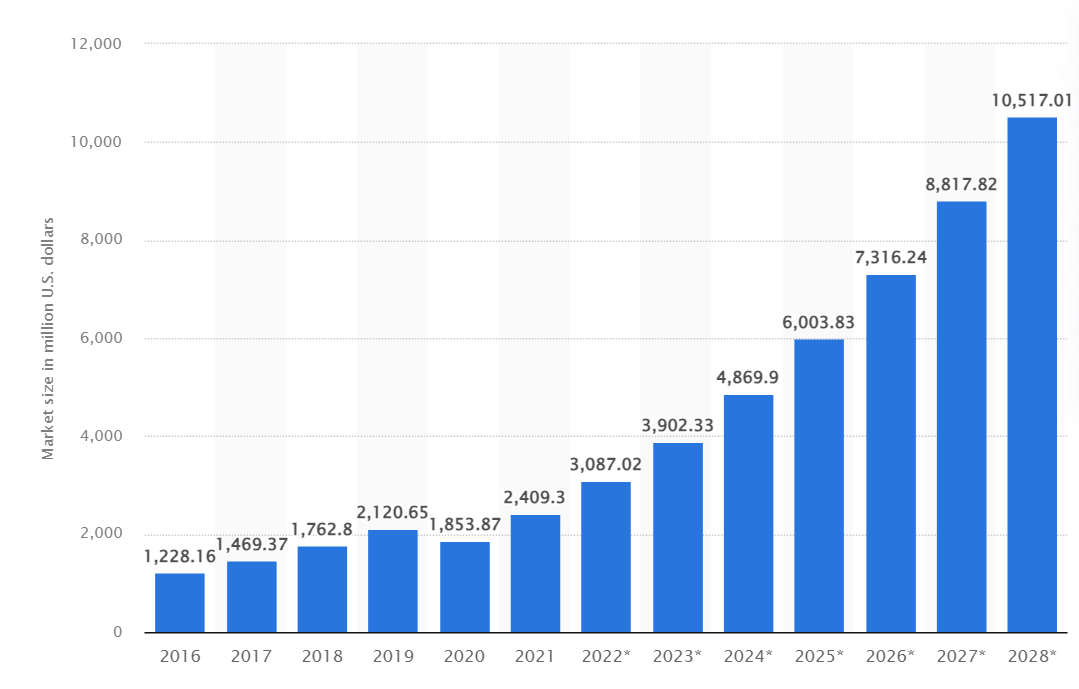
\includegraphics[width=0.9\textwidth]{mercado_robo}\\
    }
    {\sourcecitation{\textcite{robot_market}.}}
\end{figure}

É neste contexto que se insere o projeto atual.
Utilizando o robô Twil, é proposto um sistema de navegação autônomo que utiliza
sensores para mapear o ambiente em conjunto com algoritmos de planejamento
de trajetórias para permitir a navegação sem colisões em ambientes previamente
desconhecidos ou dinâmicos.

Este robô já foi utilizado em trabalhos de conclusão de curso anteriores,
como em \textcite{petry_tcc} e \textcite{rahul_tcc}.
Porém, devido ao avanço do campo da robótica, ferramentas utilizadas
nesses trabalhos foram substituídas por novas versões, que implementam
técnicas modernas que serão abordadas ao longo do trabalho.
É o caso do ROS 2, sucessor do ROS 1, que é uma coleção de bibliotecas e
ferramentas para desenvolvimento de robôs, e do \textit{Navigation 2}, um
pacote para implementar navegação autônoma em robôs móveis, que substituí o
\textit{Navigation Stack} do ROS 1.

Neste trabalho, será dado seguimento ao desenvolvimento anterior no Twil, com
ajustes na odometria, além da adição de localização utilizando uma câmera de profundidade
e mapeamento do ambiente para permitir a navegação autônoma em ambientes dinâmicos.
Nos capítulos seguintes, é apresentado o embasamento teórico necessário para
este desenvolvimento, além do planejamento da implementação deste sistema.

\chapter{Revisão da Literatura}
\label{revisao}

% Laranja sugeriu um texto introdutório aqui...
Neste capítulo são apresentados os conceitos necessários para o desenvolvimento
do trabalho, como o Robot Operating System~(ROS) 2, árvores de comportamento, mapeamento
de ambientes e o \textit{Navigation 2}.

\section{Robot Operating System 2 (ROS 2)}

O ROS 2 é a segunda geração do Robot Operating System,
um \textit{framework} para desenvolvimento de robôs.
Ele foi desenvolvido a partir do zero para atender as necessidades de robôs modernos,
com suporte para customização extensiva.
O \textit{Data Distribution Service}~(DDS) é utilizado como o \textit{middleware},
que também é utilizado em sistemas de infraestrutura crítica, como aplicações militares,
aeroespaciais e financeiras. Este padrão confere ao ROS ótima segurança e suporte para comunicação em
tempo real~\cite{ROS2Article}.

Um assunto relevante a este trabalho são os padrões de comunicação do ROS 2.
Existem três tipos de comunicação no ROS 2: \textit{topics}, \textit{services} e \textit{actions}.
\textit{Topics} são canais de comunicação unidirecionais, em que um nó, chamado de \textit{publisher},
publica uma mensagem e outros nós, os \textit{subscribers}, podem se inscrever no tópico publicado
para receber essa mensagem.
\textit{Services} são um mecanismo do tipo \textit{remote procedure call}~(RPC),
em que um nó faz uma chamada a outro nó que executa uma computação e retorna um resultado,
funcionando como um cliente e um servidor.

\textit{Actions}, são utilizados para tarefas de longa duração, com possibilidade de
cancelamento prematuro.
O cliente começa a execução enviando uma requisição para o servidor,
que response periodicamente com o estado atual da tarefa.
No término, é enviado o resultado, podendo ser sucesso ou falha.
Um exemplo de uso é uma tarefa de navegação em que um \textit{action client}
envia uma requisição com um ponto de destino para um \textit{action server}
que responde com realimentação contínua da posição atual do robô e
com o resultado ao finalizar a tarefa.
Eles também são apropriados para utilização em árvores de comportamento.

\section{Árvores de comportamento}
\todo[]{Eu comentei essa seção porque achei desnecessária, já que eu não mexi nas
    arvores de comportamento do nav2}

% Árvores de comportamento, em inglês \textit{behavior trees}~(BT), foram desenvolvidas
% na indústria de jogos para aplicação em inteligência artificial de personagens
% não jogáveis, substituindo máquinas de estado.
% Elas se destacam por sua modularidade e reatividade, porém, mantendo as funcionalidades
% esperadas de uma máquina de estado~\cite{BehaviorTree}.

% O funcionamento de uma árvore de comportamento ocorre através de uma série de
% sinais enviados aos nós de uma árvore com uma frequência fixa.
% Este nó responde com o estado atual da execução, que pode ser \textit{running},
% se está em execução, \textit{success}, se atingiu o objetivo, ou \textit{failure}
% nos demais casos.
% Na formulação clássica, existem quatro categorias de nós de controle (\textit{Sequence},
% \textit{Fallback}, \textit{Parallel} e \textit{Decorator}) e duas categorias
% de nós de execução (\textit{Action} e \textit{Condition}).
% A Tabela \ref{tab:bt_nodes} mostra os símbolos utilizados para representar
% os nós de uma árvore de comportamento.

% % LTeX: enable=false
% \begin{table}[h]
%     \begin{center}
%         \caption{Símbolos dos nós de uma árvore de comportamento.}
%         \label{tab:bt_nodes}
%         \begin{tabular}{cc}
%             Tipo de nó         & Símbolo                    \\                    %& Sucesso                             & Falha                                & Executando                     \\
%             \hline
%             \textit{Fallback}  & \fbox{?}                   \\                   %& Se um filho retorna sucesso         & Se todos filhos retornam falha       & Se um filho retorna executando \\
%             \textit{Sequence}  & \fbox{$\rightarrow$}       \\       %& Se todos filhos retornam sucesso    & Se um filho retorna falha            & Se um filho retorna executando \\
%             \textit{Parallel}  & \fbox{$\rightrightarrows$} \\ %& Se $\geq M$ filhos retornam sucesso & Se $ > N - M$ retornam falha         & Nos outros casos               \\
%             \textit{Action}    & \fbox{texto}               \\               %& Se atinge o objetivo                & Se não é possível atingir o objetivo & Durante execução               \\
%             \textit{Condition} & \ovalbox{texto}            \\            %& Se é verdade                        & Se é falso                           & Nunca                          \\
%             \textit{Decorator} & $\Diamond$                 \\                 %& Customizado                         & Customizado                          & Customizado                    \\
%             \hline
%         \end{tabular}
%     \end{center}
%     {\sourcecitation{Autor}}
% \end{table}
% % LTeX: enable=true

% O resultado dos nós de controle dependem dos resultados de seus nós filhos.
% Por exemplo, o nó \textit{Sequence} executa seus filhos em ordem até encontrar um
% nó que retorna \textit{failure} ou \textit{running}.
% Caso não encontre, retorna \textit{success}.
% O nó \textit{Fallback} funciona de forma semelhante porém procura filhos que retornem
% \textit{success} ou \textit{running}, só retornando \textit{Failure}, caso contrário.
% O nó \textit{Parallel}, executa todos os filhos em paralelo, com o resultado dependendo
% do estado de execução dos filhos.
% O nó \textit{Decorator} modifica o resultado de um nó filho de acordo com uma regra
% definida pelo usuário.

% O nó de execução \textit{Action} executa um comando, e retorna o resultado final deste comando,
% como \textit{sucess} caso o objetivo seja atingido, ou \textit{failure}, caso contrário.
% Enquanto a tarefa está sendo executada, o nó retorna \textit{running}.
% Finalmente, o nó \textit{Condition} testa uma condição e retorna
% \textit{success} ou \textit{failure}, se o resultado
% for verdadeiro ou falso, respectivamente.

% Estes nós podem ser combinados para facilmente criar comportamentos
% procurados em robôs, como mostra a Figura \ref{fig:bt_exemplo},
% que descreve a operação de \textit{pick-and-place} de um robô manipulador móvel,
% utilizando os nós \textit{Fallback}, \textit{Condition},
% \textit{Sequence} e \textit{Action}.

% \begin{figure}[h]
%     {
%         \centering
%         \caption{Exemplo de árvore de comportamento de um robô manipulador móvel.}
%         \label{fig:bt_exemplo}
%         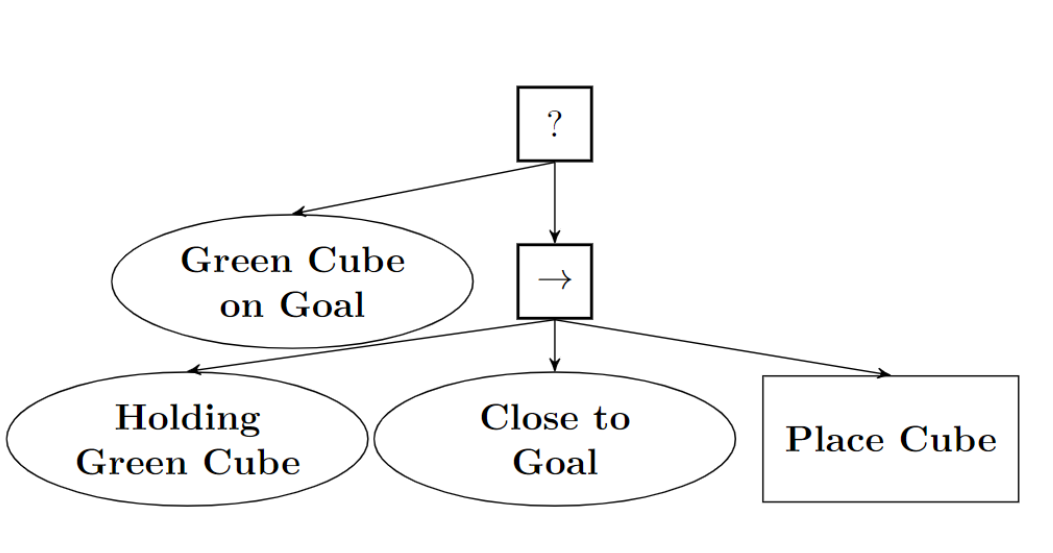
\includegraphics[width=0.5\textwidth]{bt_exemplo.png}\\
%     }
%     {\sourcecitation{\textcite{BehaviorTree}.}}
% \end{figure}

% Como permitem a construção destes comportamentos de forma visual, sem a
% necessidade de programação, árvores de comportamento estão sendo cada
% vez mais utilizadas em projetos de robótica. Exemplos de produtos
% reais são o robô JIBO e o projeto iQmatic da Scania, que
% utiliza árvores de comportamento no sistema de navegação de caminhões
% autônomos~\cite{BehaviorTree}.

\section{Mapeamento}

Para navegação autônoma, o robô deve ter conhecimento prévio do ambiente
para planejamento de trajetórias.
Existem diversas formas de representação do ambiente,
como mapas de gradientes, mapas de custo e vetores de espaços.
Neste trabalho, o foco será no mapa de custo.

O mapeamento também auxilia na localização do robô, comparando o mapa construído
com os dados dos sensores em tempo real. Além disso, os dados dos sensores podem ser
utilizados para atualizar o mapa de custo, em casos de ambientes pouco conhecidos ou dinâmicos.

É possível utilizar os dados de localização e dos sensores para construir um novo mapa.
Esta técnica é conhecida como \textit{Simultaneous Localization and Mapping~(SLAM)},
que permite a criação de mapas para ambientes pouco ou não conhecidos.

\subsection{Mapas de custo}
\todo[inline]{Isso deveria ser uma seção e não uma subseção.
    Nas subseções poderiam ter os plugins/camadas}

Um mapa de custo é uma representação de ambiente composta por uma
grade de células que contém um valor, variando de desconhecido, livre,
ocupado ou custo inflado.

Em mapas de custo tradicionais, seus dados são armazenadas em mapas monolíticos,
para utilização em planejamento de trajetórias.
Esta implementação é utilizada com sucesso para caminhos curtos,
mas pode apresentar dificuldade em lidar com ambientes dinâmicos
maiores~\cite{layered_costmaps}.

% Laranja pediu referencias para esta parte
Uma solução para este problema são mapas de custo com camadas,
que separam o processamento dos dados dos mapas de custos em camadas semanticamente distintas.
Por exemplo, os dados dos sensores e o mapa estático previamente conhecido são processados
em camadas separadas e depois combinados em um único mapa de custo.
A Figura \ref{fig:mapa_camadas} mostra uma configuração possível de camadas
de mapas de custo.
\todo[inline]{colocar que a figura é traduzida/adaptada}
\todo[]{colocar mais referencias(Laranja recomendou)}

\begin{figure}[h]
    {
        \centering
        \caption{Exemplo de configuração de camadas de um mapa de custo.}
        \label{fig:mapa_camadas}
        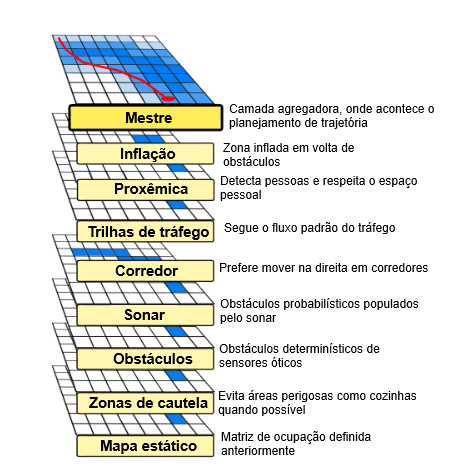
\includegraphics[width=0.5\textwidth]{mapa_camadas_trad.png}\\
    }
    {\sourcecitation{Adaptado de \textcite{layered_costmaps}.}}
\end{figure}
\subsection{Sensores e SLAM}

A escolha do sensor é importante para o mapeamento,
pois afeta a qualidade e quantidade de informações obtidas pelo robô, além
de determinar a escolha das ferramentas utilizadas para o mapeamento do
ambiente~\cite{SensorAndSLAM}.

Sensores acústicos, como sonares e sensor de óticos, são utilizados
em ferramentas SLAM 2D tradicionais. Estes sistemas são robustos e bem estabelecidos,
com fácil integração ao sistema de navegação do ROS 2.

Porém, com o avanço da tecnologia, sensores Red Green Blue - Depth~(RGB-D)
e câmeras estéreo estão se tornando mais acessíveis, influenciando o
desenvolvimento de sistemas de Visual~SLAM~(VSLAM).
Dentre sistemas de VSLAM, destacam-se o ORB-SLAM3, OpenVSLAM e RTABMap, que possuem suporte
a câmeras RGB-D e permitem localização pura.
Em \textcite{VSLAM}, é feita uma comparação entre estes sistemas, mostrando que o
OpenVSLAM é a técnica mais adequada para maioria dos casos.
Contudo, para ambientes internos com câmeras RGB-D, o RTABMap também teve um bom desempenho.
Estes sistemas, porém, não são integrados nativamente ao \textit{Navigation2}.

\todo{Falar mais do slam/vslam eu acho}
% TODO: Procurar artigos mais novos sobre VSLAM (o referenciado ta na pagina
% do nav2, mas parece estar desatualizado...)
% O NVidia Isaac ROS VSLAM e o StellaROS(parece que é uma continuacao do OpenVSLAM)
% parecem promissores...

\section{Navigation2}

O \textit{Navigation2}~(Nav2) é o sucessor do ROS \textit{navigation stack}, permitindo
a realização de tarefas complexas em diversos ambientes e classes de robôs cinemáticos.
Baseando-se no legado do \textit{navigation stack} do ROS 1, o Nav2 foi construído em cima
do ROS2, implementando técnicas mais modernas para ter um sistema modular propício para
ambientes dinâmicos com suporte a uma maior variedade de sensores~\cite{Nav2}.

Uma árvore de comportamento é utilizada para
orquestrar as tarefas de navegação, ativando os servidores de controle, planejamento e
recuperação para navegação.
Para executar nós de \textit{actions}, são normalmente utilizados
\textit{Action servers} do ROS 2.
Esta árvore de comportamento pode ser configurada pelo usuário através de um arquivo
em XML, permitindo a descrição de comportamentos de navegação únicos sem
necessidade de programação.

Além disso, todos estes servidores utilizam o conceito de \textit{Managed Nodes},
também conhecidos como \textit{Lifecycle Nodes}.
Estes nós utilizam máquinas de estados para gerenciar seu ciclo de vida, utilizando
transições de estado desde sua criação a destruição.
No caso de falha ou desligamento, o nó vai do estado ativo ao estado finalizado,
seguindo a máquina de estados, permitindo que o sistema seja interrompido
de forma segura.

Na arquitetura pode-se notar a utilização de dois mapas de custo, um local e
outro global.
O mapa local, utilizado no servidor do controlador, realiza o planejamento
a curto prazo e prevenção de colisão, enquanto o mapa global,
aplicado no servidor de planejamento, é usado principalmente
para planejamento a longo prazo.

\chapter{Metodologia}
\label{desenvolvimento}

Utilizando ferramentas da versão Humble do ROS 2, foi desenvolvido um sistema de
navegação autônoma para o robô Twil, que utiliza uma câmera RGB-D Intel RealSense D435
para mapeamento do ambiente.
Dentre as ferramentas utilizadas, destacam-se o Gazebo, utilizado para simulação do robô,
e o \textit{Navigation2}, que fornece diversas ferramentas para implementar
e orquestrar um sistema de navegação autônoma.

Os variados componentes do robô, como os sensores utilizados neste trabalho,
foram implementados através de \textit{plugins} do Gazebo,
que comunicam o estado do robô durante a simulação através de tópicos do ROS 2.

\todo[inline]{
    explicar melhor a arquitetura do nav2 aqui

    a imagem da arquitetura não é muito boa, entao precisa de uma explicacao geral melhor

    é uma boa explicar o que faz o servidor de controlador(define a velocidade do robo pra
    seguir a trajetoria), já que é utiliza outro contrador para transformar a velocidade
    em comandos para as rodas do robo
}

O \textit{Navigation2}, que tem sua arquitetura mostrada na Figura
\ref{fig:nav2_arc}, foi configurado para utilizar estes componentes.
O \textit{Nav2} é responsável pelo envio comandos de velocidade para o robô, para que ele chegue
ao destino desejado de modo seguro, evitando colisões.
Para isso, são necessários: uma representação do ambiente, a posição do robô neste ambiente e
um controlador para transformar os comandos de velocidade em comandos para as rodas do robô.

A representação do ambiente é feita através de um mapa de custo, e é onde o servidor do planejador
se baseia para construção de trajetórias seguras do robô.
A posição do robô é obtida através de transformações entre os sistemas de coordenadas \texttt{map},
\texttt{odom} e \texttt{base\_link} do robô, conforme a especificação REP 105~\cite{rep_105}.
Esta posição é utilizada pelo servidor de controlador para gerar comandos de velocidade conforme
a trajetória planejada.

\begin{figure}[h]
    {
        \centering
        \caption{Arquitetura do \textit{Navigation2}.}
        \label{fig:nav2_arc}
        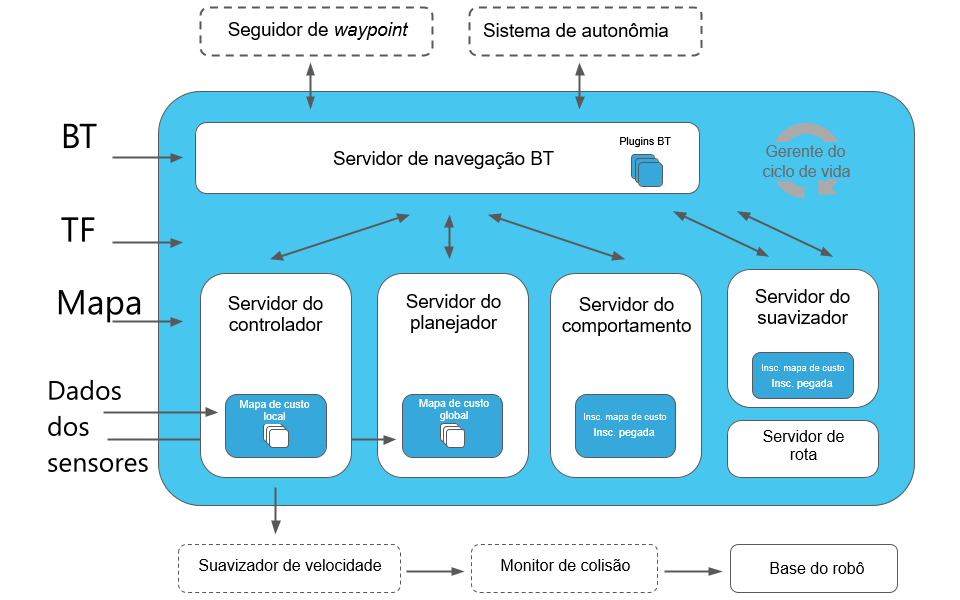
\includegraphics[width=0.9\textwidth]{nav2_architecture_trad.png}\\
    }
    {\sourcecitation{Adaptado de \textcite{nav2_site}.}} % colocar adaptado/traduzido?
\end{figure}

Antes do início deste trabalho, o Twil já estava configurada para utilizar o \textit{Nav2},
porém sem utilizar dados da câmera e IMU.
Portanto, as trajetórias planejadas não eram atualizadas
para evitar obstáculos e não havia sistema de localização, ou seja,
a transformada entre \texttt{map} e \texttt{odom} era estática, portanto
não havia ajuste da odometria implementada.

Em razão disso, foi adicionada a câmera RGB-D Intel RealSense D435 e um IMU ao robô,
e o sistema de navegação foi aprimorado com a utilização destes sensores nos
de odometria, localização e mapeamento.

\todo[inline]{
    no diagrama simplificado,
    optei por nao colocar uma seta da localizacao para camada voxel,
    mas é claro que precisa da posicao do robo, só que ele usa a localizacao do nav2,
    entao isso foi configurado "implicitamente"
    (eu também achei que essa seta ia poluir muito o diagrama)}

Um diagrama simplificado da arquitetura do trabalho é mostrado na
Figura \ref{fig:arq_trabalho}.
Neste trabalho, todos sistemas conectados a câmera e o IMU foram modificados.
O desenvolvimento deste trabalho foi focado nos componentes em vermelho
e verde, que utilizam os dados da câmera.
Em vermelho, estão os componentes referentes ao mapeamento do ambiente,
onde são criados dois mapas.
O primeiro mapa é um mapa de custo utilizado no planejamento de trajetórias,
onde foi adicionada uma camada para percepção de obstáculos utilizando
a câmera RGB-D, além da calibração da camada de inflação.
O segundo mapa é criado e utilizado pelos sistemas de localização do robô.
Em verde, estão os componentes referentes a estimativa de
posição do robô, onde foram adicionados pacotes que realizam a
odometria visual e pacotes de SLAM.
\todo{apesar de eu ter adicionado a fusao, no final nao mudou nada na odometria,
    talvez seja melhor nem mencionar}
Também foi realizado ajustes na odometria das rodas, através da fusão
de dados com o sensor IMU.
Para testes, foi mantida a opção de utilizar a transformada estática entre
\texttt{map} e \texttt{odom}, e foi adicionado um sistema de odometria
utilizando a posição exata do robô no Gazebo.

\begin{figure}[h]
    {
        \centering
        \caption{Arquitetura do simplificada do trabalho.}
        \label{fig:arq_trabalho}
        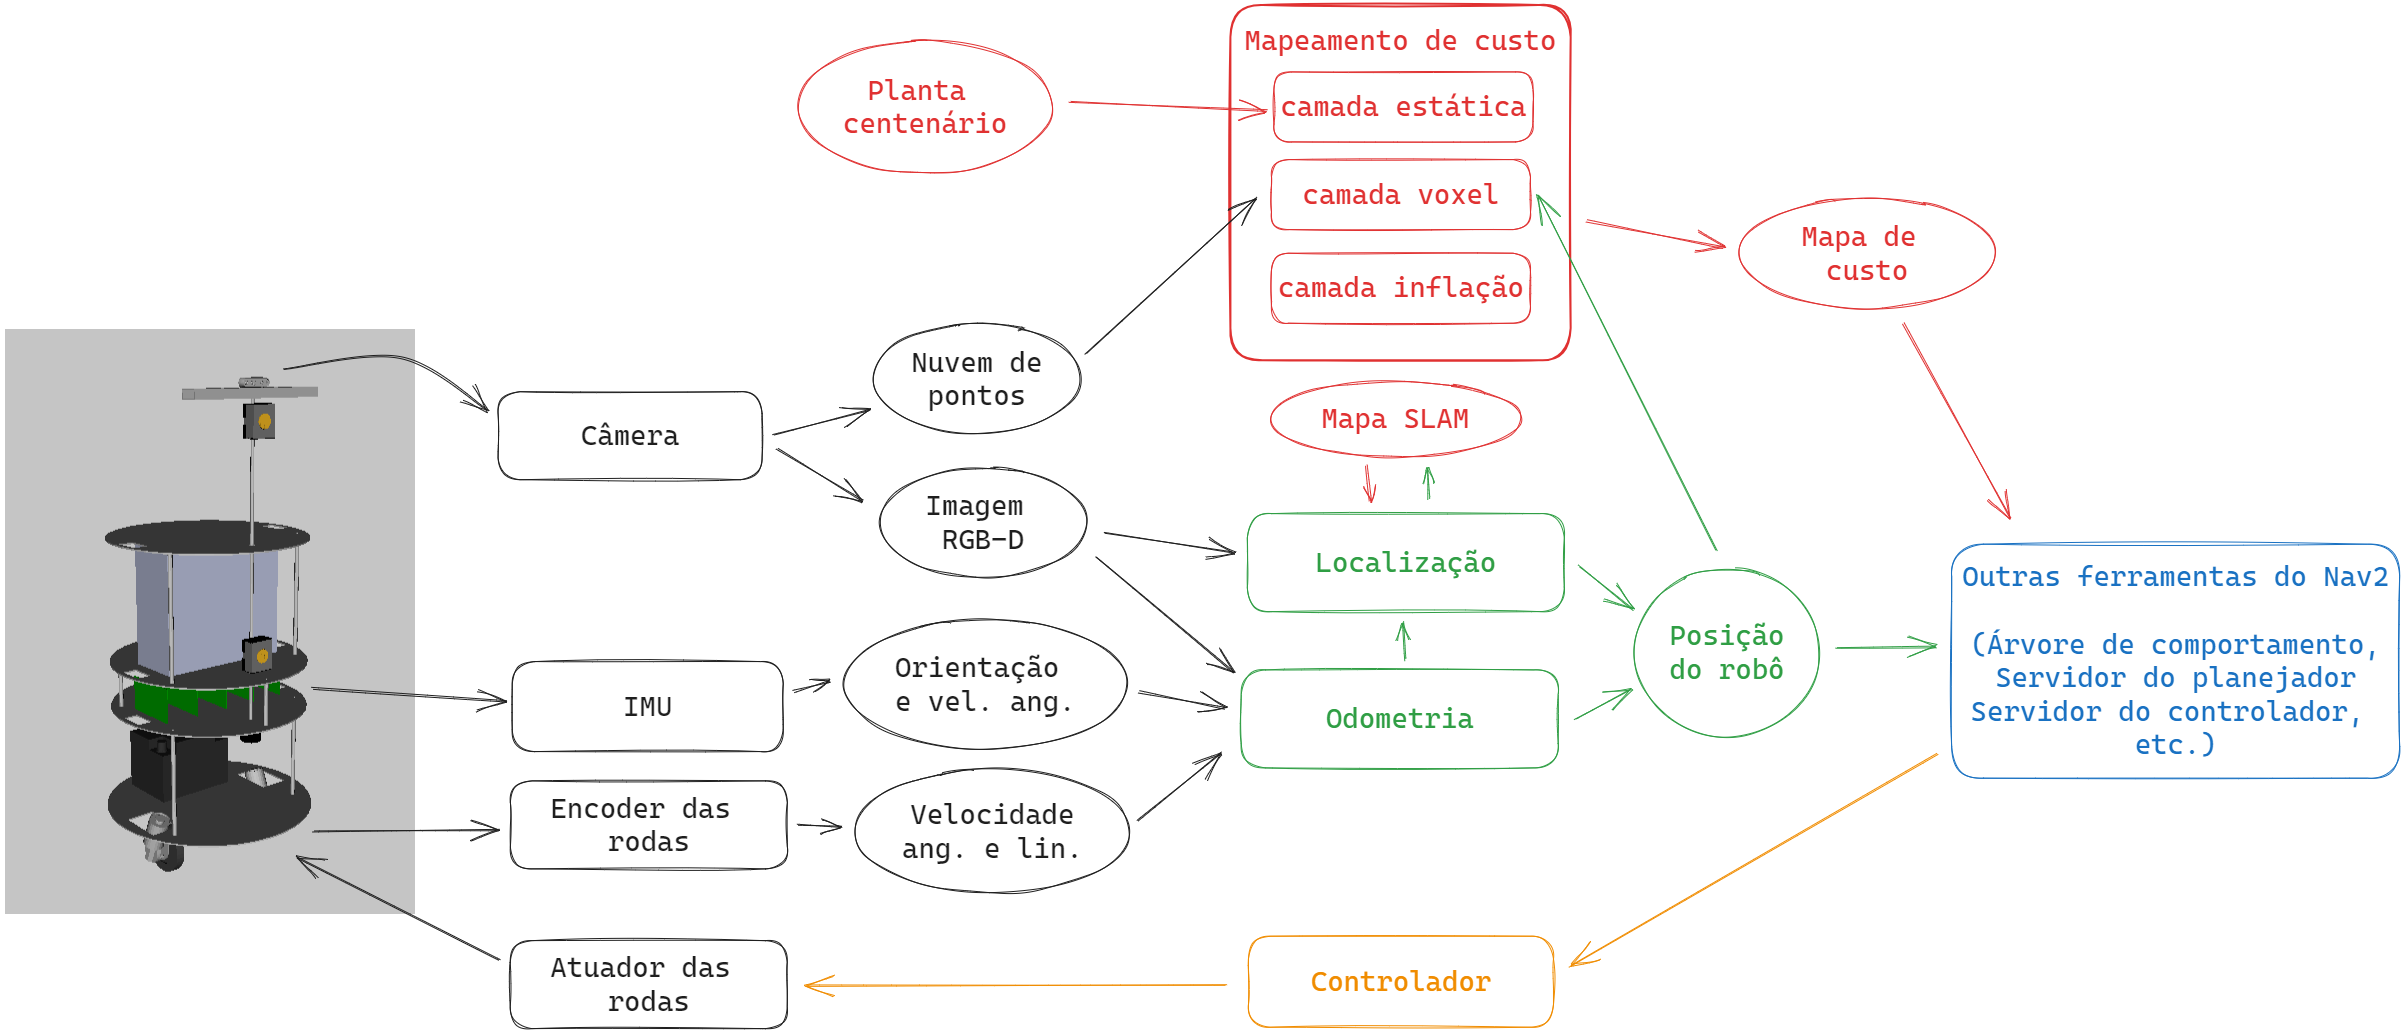
\includegraphics[width=0.98\textwidth]{arquitetura_simplificadav3.png}\\
    }
    % {\sourcecitation{Autor.}}
\end{figure}

Nas seções seguintes, será apresentado o robô e o ambiente de testes
utilizado neste trabalho.
Em seguida, será detalhado o desenvolvimento dos sistemas necessários
para a navegação autônoma do robô neste ambiente.
Finalmente, será descrita a coleta de dados para a análise dos resultados,
que é apresentada no próximo capítulo.

\section{Configuração do robô}


\todo[inline]{
    foi retirada uma roda e a bateria foi movida para tras, mas nao mudou nada,
    entao nao sei se coloco
}

O modelo do robô está presente no pacote \texttt{twil\_description}, que contém
os arquivos de descrição do robô no formato XACRO, que é compilado para o formato
URDF, utilizado pelo ROS 2.
Este modelo é utilizado no rviz para visualização do robô, além de ser utilizado
no Gazebo para simulação.
Para a simulação dos componentes físicos do robô, como sensores e atuadores,
são utilizados \textit{plugins} do Gazebo.

Durante este trabalho, foram configurados dois novos componentes ao robô, a câmera
RGB-D Intel RealSense D435 e um IMU.
A câmera foi utilizada nos sistemas de odometria, localização e mapeamento,
enquanto o IMU foi utilizado para melhorar a qualidade da odometria,
fornecendo dados de orientaçao do robô.

Para utilização da câmera, é necessário o pacote
\texttt{realsense-ros}~\cite{realsense_ros}, que contém o modelo da câmera.
O \textit{plugin} do Gazebo \texttt{camera\_plugin},
é responsável pela publicação dos dados da câmera simulada.
São utilizados cinco tópicos para publicar estes dados:
\todo{talvez faça mais sentido colocar o tipo de msg, ou só explicar os tópicos}
\texttt{/camera/color/image\_raw}, \texttt{/camera/color/camera\_info},
\texttt{/camera/depth/image\_raw}, \texttt{/camera/depth/camera\_info} e
\texttt{/camera/infra1/image\_raw}.

A adição do IMU foi feita utilizando o \textit{plugin}
\texttt{GazeboRosImuSensor}, que publica mensagens do tipo
\texttt{sensor\_msgs/Imu}.
Estas mensagens contém a orientação, velocidade angular e aceleração linear do robô.
Por si só, o IMU não é confiável para estimar a posição do robô, porém, estes
dados podem ser fundidos com outras fontes de odometria para melhorar a
acurácia da estimativa de posição.
Como o modelo físico do IMU, foi reutilizada
a descrição da placa de circuito impresso \textit{Eurocard},
que já era utilizada em outros componentes do robô.

A conversão dos comandos de velocidade em movimento de rodas do
robô é feita pelo controlador, executado pelo \texttt{twil\_bringup},
que utiliza o controlador \textit{twist\_mrac\_controller},
presente no pacote \texttt{linearizing\_controllers}.
Este controlador foi configurado em trabalhos anteriores para
ser utilizado com o \textit{Navigation2}.
O pacote \texttt{arc\_odometry} é executado junto por este
controlador para transformar os dados de posição das juntas
da roda em mensagens do tipo \texttt{nav\_msgs/Odometry},
que publicam a posição, orientação e velocidades do robô em relação
ao sistema de coordenadas \texttt{odom}.

\section{Ambiente de simulação}

O sistema será simulado em uma simulação do prédio Centenário da Escola de Engenharia
da UFRGS, utilizando o Gazebo, como em trabalhos anteriores.
No pacote \texttt{ufrgs\_map} está incluído uma representação em formato PGM da
planta do prédio, mostrada na Figura \ref{fig:planta_centenario}, desenvolvida em
trabalhos anteriores.
Além da imagem da planta, também está presente um arquivo de configuração
em formato YAML, que contém a resolução, origem do mapa.
Como este mapa é utilizado como mapa de custo, este arquivo de configuração
também contém parâmetros de configuração
que definem os valores que indicam se uma célula está livre ou ocupada.
\todo{essa ultima frase ta terrível}

\begin{figure}[h]
    {
        \centering
        \caption{Planta do 1º andar do prédio Centenário da EE-UFRGS.}
        \label{fig:planta_centenario}
        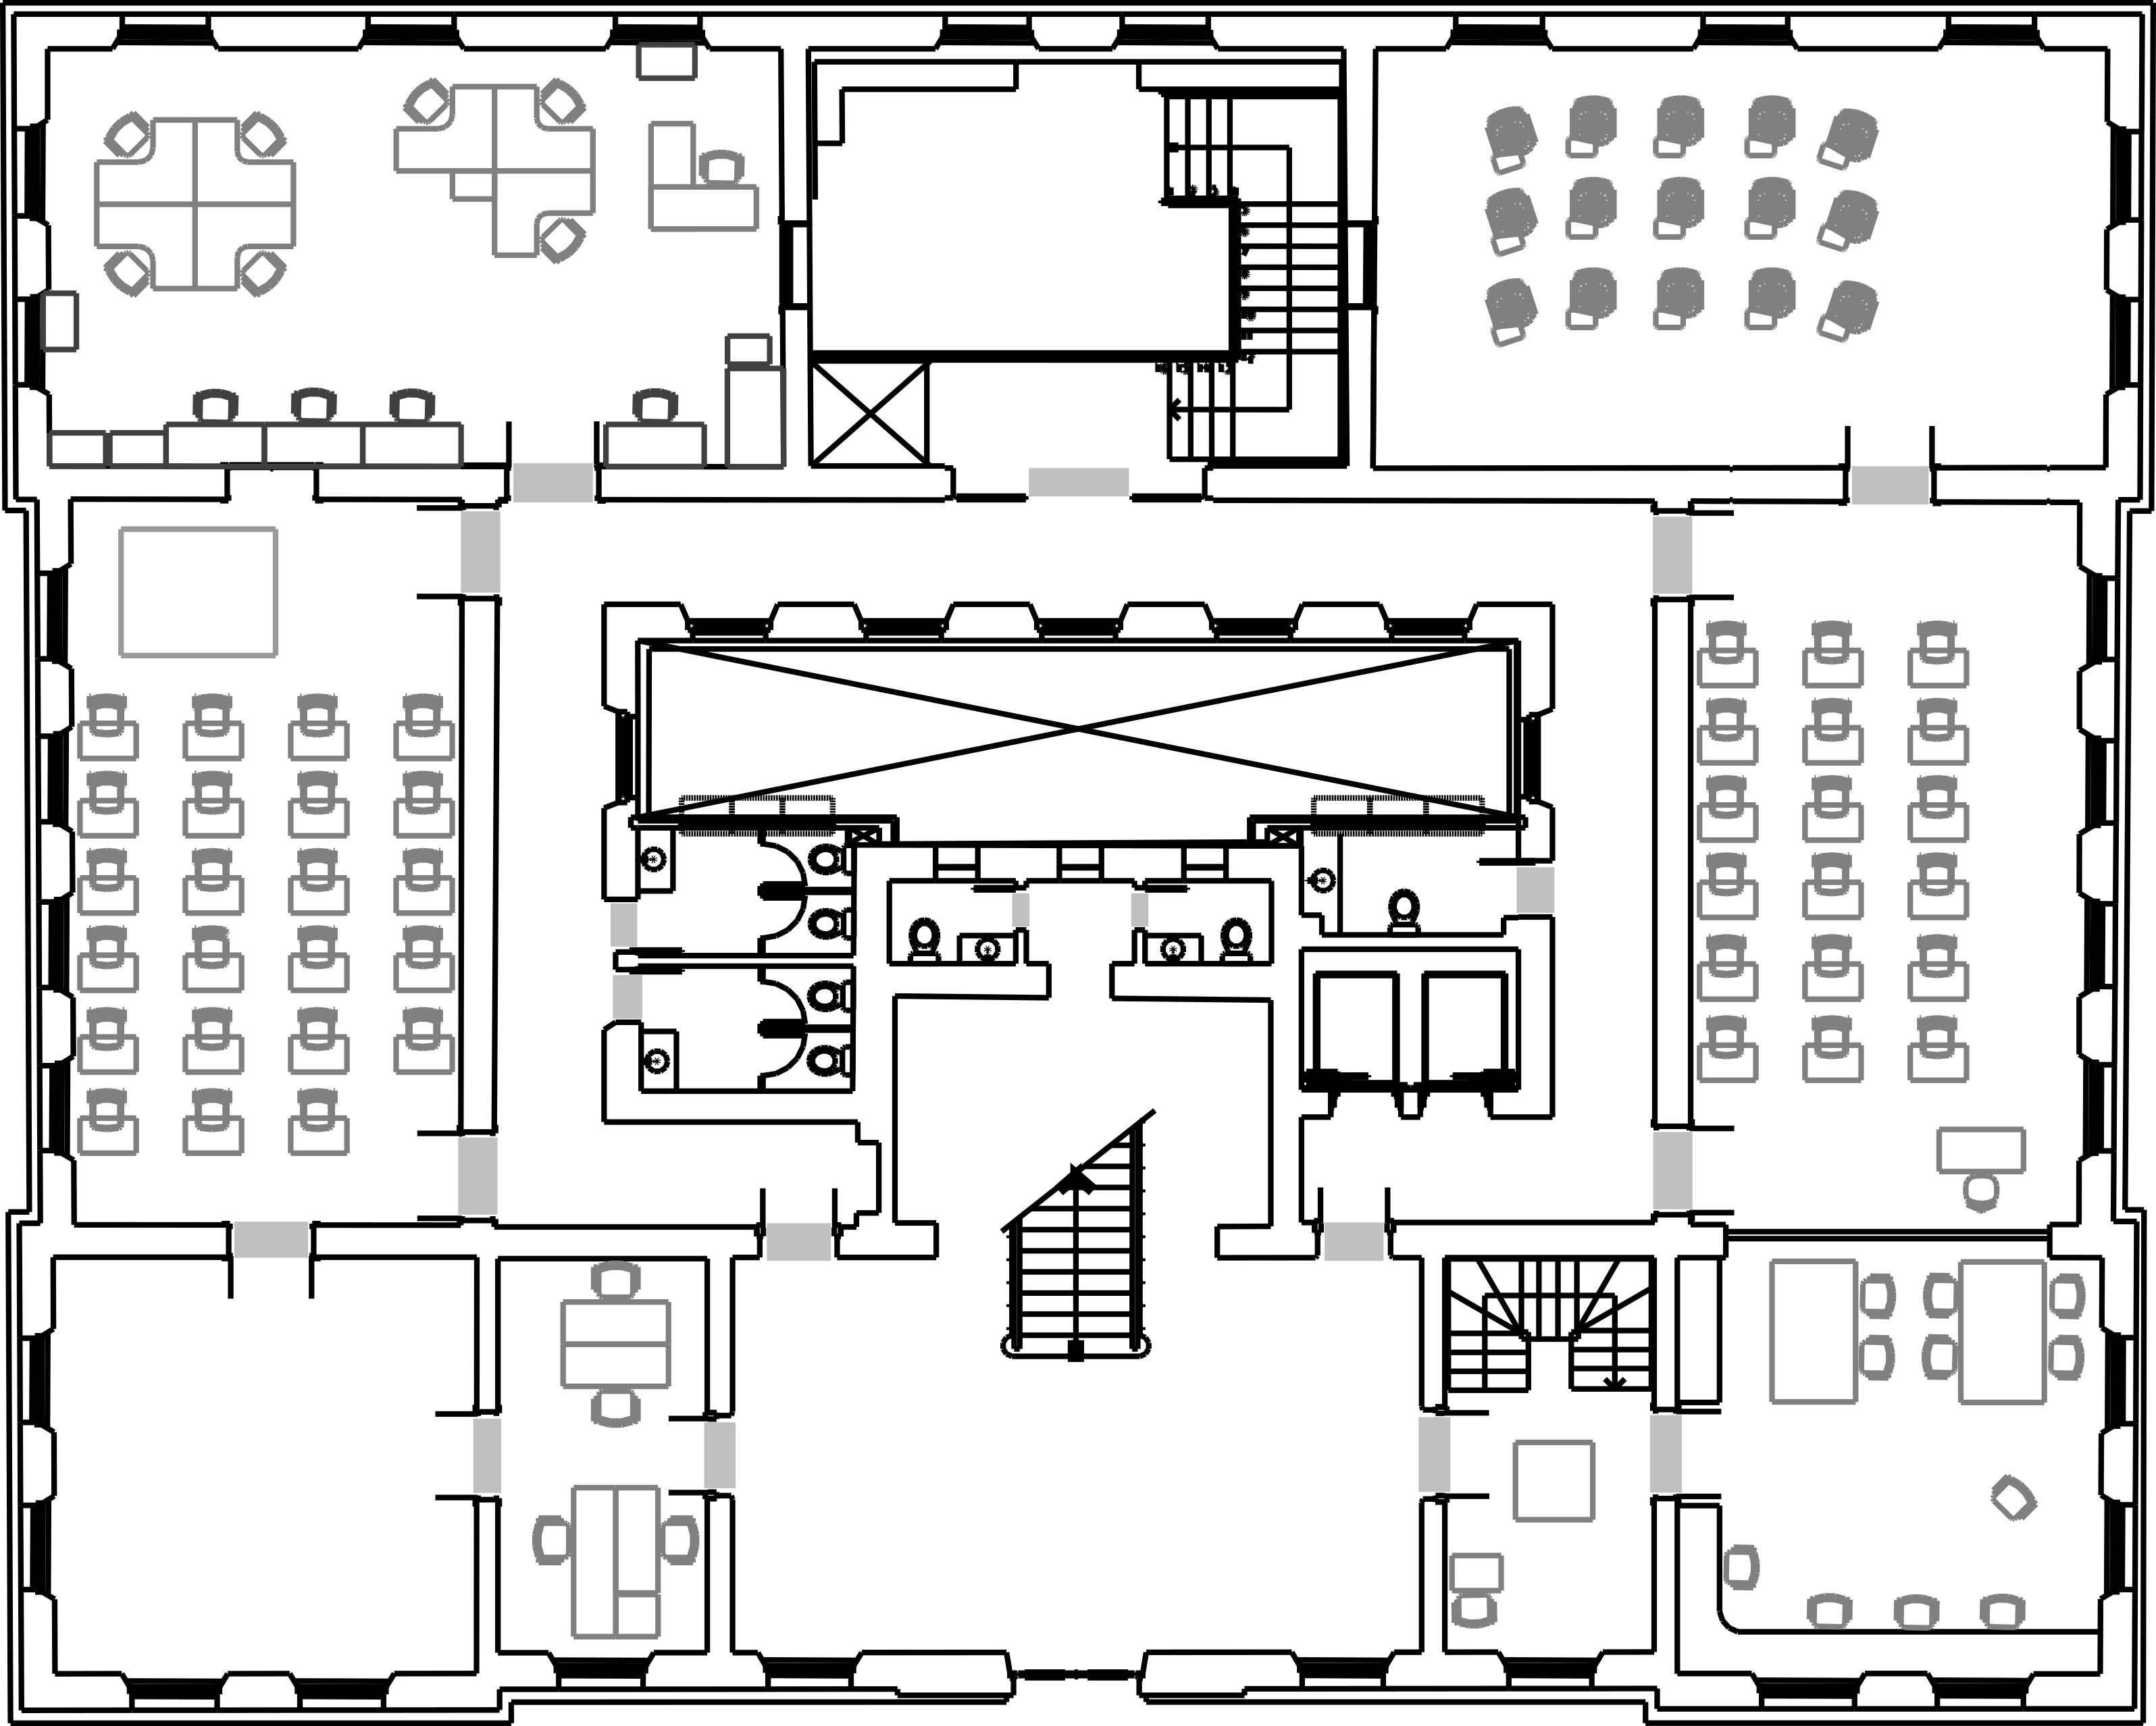
\includegraphics[width=0.5\textwidth]{centenario_floor_plan.png}\\
    }
    {\sourcecitation{\textcite{petry_tcc}.}}
\end{figure}

O pacote \texttt{ufrgs\_gazebo} contém arquivos de mundos do Gazebo para
simulação.
Este pacote, porém, estava desatualizado e não continha uma representação do
prédio Centenário.
Utilizando o \textit{Building Editor} do Gazebo, foi criado um modelo do prédio
em 3D, com base na planta do prédio, mostrado na Figura \ref{fig:gazebo_centenario}.
\todo{será que escrevo sobre a textura das paredes?}

\begin{figure}[h]
    {
        \centering
        \caption{Ambiente Gazebo com modelo do prédio Centenário da EE-UFRGS.}
        \label{fig:gazebo_centenario}
        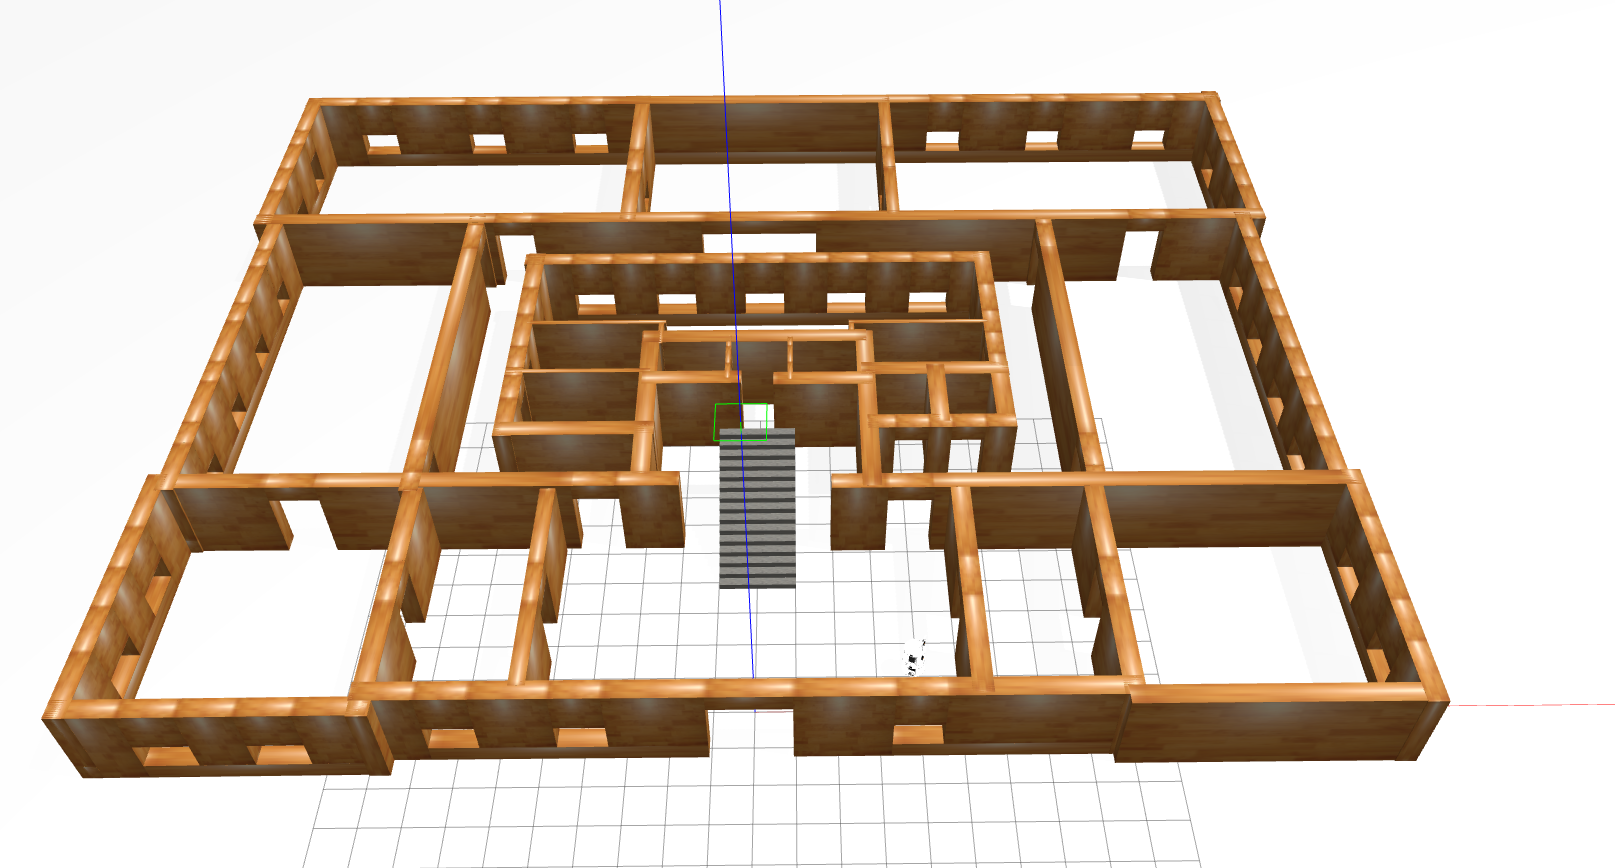
\includegraphics[width=0.9\textwidth]{gazebo.png}\\
    }
    % {\sourcecitation{Autor.}}
\end{figure}

Para testar a prevenção de colisões com obstáculos dinâmicos, são
adicionados objetos padrões do Gazebo, como caixas e cilindros,
durante a simulação neste ambiente.

\section{Odometria e localização}

A estimativa de posição é feita utilizando o sistemas de coordenadas definido pela
norma REP 105~\cite{rep_105}, que define quatro sistemas de coordenadas: \texttt{earth},
\texttt{map}, \texttt{odom} e \texttt{base\_link}.
Como só é utilizado um mapa, o sistema de coordenadas \texttt{earth} não será utilizado.
Todas transformadas entre estes sistemas de coordenadas são
publicadas no tópico \texttt{/tf}.

O sistema de odometria é responsável pela publicação da transformada entre o sistema
de coordenadas \texttt{odom} e \texttt{base\_link}.
A posição do robô em relação ao \texttt{odom} deve ser contínua, porém pode divergir
gradualmente. Por esta razão, são geralmente utilizados sensores incrementais na
odometria, que estimam a posição e orientação do robô por integração e, portanto,
são suscetíveis a erros de acumulação.

Neste trabalho, serão utilizados e comparados três sistemas de odometria,
que além da transformada, também publicam mensagens do tipo
\texttt{nav\_msgs/Odometry} no tópico \texttt{/odom}.
Antes deste trabalho, a odometria era publicado pelo controlador,
através do pacote \texttt{twist\_mrac\_controller}, utilizando
dados do encoder nas rodas para estimar a posição do robô.
O cálculo da posição é feito pelo pacote \texttt{arc\_odometry}, que utiliza
o modelo cinemático de um robô móvel de acionamento diferencial
para estimar a posição e orientação do robô.
Para aprimorar a qualidade desta odometria, foi adicionado o pacote
\texttt{robot\_localization}, que realiza a fusão de
de dados da odometria das rodas com os dados do IMU.

A fusão é realizada através de um filtro de Kalman estendido, onde devem
ser escolhidos quais dados dos sensores devem ser considerados.
Apesar da recomendação de configuração dos criadores do pacote, onde é
sugerido utilizar apenas dados de velocidade e não de posição,
para os dados calculados pelo \texttt{arc\_odometry}, decidiu-se utilizar
tanto a posição quanto a velocidade na fusão de dados.
Isso foi feito porque a velocidade calculada pelo \texttt{arc\_odometry}
é calculada em referência ao sistema de coordenadas global, neste caso, o \texttt{odom},
enquanto que o \texttt{robot\_localization} espera que a velocidade seja em referência
a base do robô.
Desta forma, a posição publicada pelo \texttt{robot\_localization} é a mesma que a
publicada pelo \texttt{arc\_odometry}, já que não foram utilizados outros dados de posição.
Porém, a orientação e velocidade angular da odometria das rodas são fundidas com os dados
do IMU, melhorando a precisão apenas destes dados.


Como alternativa a este sistema, foi implementado um sistema de odometria visual,
publicado pelo executável \texttt{rgbd\_odometry} do pacote
\texttt{rtabmap\_odom}, que utiliza dados da câmera RGB-D com
o sensor IMU para estimava da posição.
Utilizando
\todo{eu traduzi "features" para caracteristicas, mas talvez seja um termo especifico de visao computacional}
características das imagens RGB, com a informação de profundidade
da imagem de profundidade, é utilizado o método RANSAC, acrônimo de
\textit{Random Sample Consensus}, para comparar imagens consecutivas e estimar
a velocidade do robô.
\todo{referenciar}
%https://wiki.ros.org/rtabmap_odom#rgbd_odometry
\todo[inline]{ explicaçao de odometria visual usando ransac que encontrei:

    doi: 10.1109/IMTIC.2018.8467263}

É possível, também, fundir os dados destes dois sistemas de odometria,
porém, optou-se por mantê-los separados para facilitar a comparação
do desempenho entre eles.

Finalmente, para realização de testes, foi implementado um sistema de odometria
\todo{será que eu deixo as aspas entre perfeito aqui?}
“perfeito”.
Utilizando o \textit{plugin} P3D do Gazebo, é publicada a posição
do robô em relação ao sistema de coordenadas \texttt{odom} como uma mensagem
do tipo \texttt{nav\_msgs/Odometry} em um tópico chamado \texttt{fake\_odom}.
Esta mensagem é retransmitida para o tópico \texttt{/odom} e utilizada pelo
pacote \texttt{odom\_to\_tf\_ros2} para publicar a transformada entre
\texttt{odom} e \texttt{base\_link}.

\todo[inline]{
    tenho que explicar em algum lugar que esse fake odom
    é diferente do ground truth porque o ground truth é em relacao ao
    map e o fake odom é em relacao ao odom
}

\begin{table}[h]
    \begin{center}
        \caption{Sistemas de odometria}
        \label{tab:odometria}
        \begin{tabular}{c|c|c}
            Pacote utilizado                              & Fonte de dados          & Tipo de mensagem recebida                       \\
            \hline
            \multirow{2}{*}{\texttt{robot\_localization}} & Encoder das rodas       & \texttt{nav\_msgs/Odometry}                     \\
                                                          & IMU                     & \texttt{sensor\_msgs/Imu}                       \\
            \hline
            \multirow{3}{*}{\texttt{rtabmap\_odom}}       & \multirow{2}{*}{Câmera} & \texttt{sensor\_msgs/CameraInfo}                \\
                                                          &                         & \texttt{sensor\_msgs/Image}(RGB e profundidade) \\
                                                          & IMU                     & \texttt{sensor\_msgs/Imu}                       \\
            \hline
            \texttt{odom\_to\_tf\_ros2}                   & Posição no Gazebo       & \texttt{nav\_msgs/Odometry}                     \\
        \end{tabular}
    \end{center}
    % {\sourcecitation{Autor}}
\end{table}
\todo[inline]{a camera no rgbd odom usa dois topicos do do tipo image,
    por isso que colocou (rgb e profundidade), mas achei que ficou estranho

    talvez faça sentido colocar o tipo de mensagem image
    duas vezes e colocar rgb numa e profundidade na outra
}

Anteriormente, nenhum sistema de localização era utilizado, e a transformada
entre \texttt{map} e \texttt{odom} era estática.
Esta transformada foi mantida para testes, e foram implementados sistemas
de localização para ajustar a odometria do robô utilizando sensores absolutos,
que não acumulam erros.
Esta transformada é publicada em uma frequência menor que a da odometria,
permitindo a utilização de sistemas de localização com alta complexidade de
processamento.

\todo[inline]{nao achei bom o prox paragrafo}

Uma opção de sistema de localização é o \texttt{nav2\_amcl}, que utiliza
\textit{Adaptive Monte Carlo Localization~(AMCL)} e um mapa estático para
estimar a posição do robô.
Porém, optou-se por utilizar sistemas de SLAM, que realizam
o mapeamento simultaneamente com a localização, já que
o objetivo é a utilização do robô em ambiente dinâmicos ou pouco conhecidos,
onde um mapa estático não seria adequado.
Além disso, a planta do prédio e o mapa do Gazebo não são idênticos, que
afeta o desempenho do sistema mesmo em situações ideais.
Portanto, dois sistemas de SLAM foram implementados,
o \textit{slam\_toolbox} e o \textit{rtabmap}.

O \textit{slam\_toolbox} realiza o SLAM em 2D, e foi criado para utilizar sensores
a laser. Portanto, são esperadas mensagens do tipo \texttt{sensor\_msgs/LaserScan}
para percepção do ambiente neste sistema. Como a câmera RGB-D não publica mensagens
desse tipo, foi utilizado o pacote \texttt{depthimage\_to\_laserscan} para converter
a imagem de profundidade da câmera na mensagem esperada, em forma de um feixe de luz
em duas dimensões localizado na altura da câmera.
O \textit{rtabmap}, por outro lado, realiza o SLAM em 3D, e utiliza todos os
tópicos publicados pela câmera RGB-D, e não necessita de conversão de mensagens.

Ambos sistemas sistemas publicam a transformada entre \texttt{map} e \texttt{odom},
além da posição global do robô no tópico \texttt{/pose}, em mensagens do tipo
\texttt{geometry\_msgs/PoseWithCovarianceStamped}, que são utilizadas para
comparação com a posição real e a estimada pela odometria.

Apesar de realizar o mapeamento do ambiente em tempo-real, estes sistemas
podem ser iniciadoscom informações de uma sessão prévia de mapeamento,
que pode aumentar a precisão da localização, caso o mapa seja mais fiel
que o construído. Porém, nos testes realizados, a sessão de SLAM foi iniciada
do zero, para simular um ambiente desconhecido.

\todo[inline]{
    talvez seja bom falar sobre o loop-closure no paragrafo anterior
}

\begin{table}[h]
    \begin{center}
        \caption{Sistemas de localização}
        \label{tab:localizacao}
        \begin{tabular}{c|c|c}
            Pacote utilizado                        & Fonte de dados          & Tipo de mensagem recebida                       \\
            \hline
            \texttt{slam\_toolbox}                  & Câmera                  & \texttt{sensor\_msgs/LaserScan}                 \\
            \hline
            \multirow{2}{*}{\texttt{rtabmap\_slam}} & \multirow{2}{*}{Câmera} & \texttt{sensor\_msgs/CameraInfo}                \\
                                                    &                         & \texttt{sensor\_msgs/Image}(RGB e profundidade) \\
            \hline
            \texttt{tf2\_ros}                       &                         &                                                 \\
        \end{tabular}
    \end{center}
\end{table}

\section{Mapeamento}

Um aspecto essencial para a navegação autônoma é a representação do ambiente.
O planejamento de trajetória necessita de um mapa do ambiente, na forma
de um mapa de custo, em que cada célula contém um valor indicando o custo
de atravessa-la. Um algoritmo de pesquisa utiliza este mapa para encontrar
a trajetória com menor custo para o destino desejado.

Apesar do sistema de SLAM fornecer um mapa do ambiente, este mapa não será
utilizado no mapa de custo. Como este mapa não está completo desde o início,
não é possível planejar trajetórias para ambientes não visitados previamente.
Além disso, o mapa pode ser criado em estados não desejados como,
por exemplo, com trajetórias bloqueadas por obstáculos temporários.

Portanto, haverão duas representações do ambiente, uma criada pelo SLAM, que
é utilizada pelo mesmo sistema para localização, e outra criada utilizando
os \textit{plugins} do mapa de custo do Nav2, que é utilizada para planejamento
de trajetória.

O mapa de custo utilizado é composto por três camadas:
\begin{enumerate}
    \item a camada estática, que possui uma representação simples do ambiente,
          sem obstáculos.
    \item a camada de obstáculos, onde são utilizados dados dos sensores óticos
          para atualizar o mapa com obstáculos dinâmicos.
    \item a camada de inflação, que cria um campo de custo ao redor dos obstáculos.
\end{enumerate}

A planta do prédio Centenário, representada na Figura \ref{fig:planta_centenario},
foi utilizada como mapa estático. O mapa foi configurado para considerar apenas as
cédulas em preto escuro como ocupados, que equivalem a obstáculos fixos, como paredes
e a escada. As cédulas em cinza claro são consideradas livres, que representam a posição
provável de objetos móveis, como cadeiras e mesas.

A camada de obstáculos utiliza os dados da camera RGB-D para atualizar o mapa.
Existem dois \textit{plugins} que podem ser utilizados para este fim, o
\texttt{obstacle\_layer} e o \texttt{voxel\_layer}.
Ambos podem utilizar mensagens do tipo \texttt{PointCloud2}, que são publicadas
pela câmera RGB-D, porém utilizam técnicas diferentes para atualizar o mapa.
\todo{nao achei traducao para ray casting}
O \texttt{obstacle\_layer} utiliza \textit{ray casting} em 2D para
determinar a posição dos obstáculos.
O \texttt{voxel\_layer}, por outro lado, cria um gride tri-dimensional,
divido em blocos chamados de \textit{voxels}, que podem estar ocupados ou livres.

Apesar do mapa de custo ser em 2D, a simulação e o mundo real podem ter obstáculos
de diferentes alturas, como mesas e cadeiras. Portanto, é necessária a percepção em
3D do ambiente para evitar colisões com estes obstáculos. Logo, foi utilizado o
\texttt{voxel\_layer} para atualizar o mapa de custo.

Para a configuração do \texttt{voxel\_layer}, é necessário definir a resolução
e o número de \textit{voxels} no eixo Z utilizados.
A câmera RGB-D Intel RealSense D435 do Twil está localizada a uma altura de aproximadamente
1,37 metros do chão, que é a altura mínima do gride de \textit{voxels}.
O número máximo de \textit{voxels} permitido pelo \textit{plugin} é 16.
Tendo em vista estes dados, foi definido um gride de \textit{voxels} com 15 \textit{voxels}
de resolução 0,1 metro, criando um gride de 1,5 metro de altura.
Portanto, serão captados obstáculos dentro deste campo, porém obstáculos com altura
superior a 1,5 metro não serão detectados.
Isso é importante para evitar a detecção de obstáculos que não são relevantes para
a navegação como, no caso do ambiente de simulação utilizado, a moldura das portas.

\todo[inline]{
    os artigos sobre o Nav2 utilizam o Spatio Temporal Voxel Layer,
    que introduz um "decay" a camada voxel

    queria usar ele mas o parece que o pacote nao foi migrado pro Humble,
    tenho que escrever isso em algum lugar
}

A última camada, \texttt{inflation\_layer}, cria uma zona de segurança ao redor
dos objetos captados nas outras camadas, para garantir uma distância segura
ao planejar a trajetória.
Em \textcite{ros_tuning_guide}, recomenda-se que a camada de inflação cubra
um raio grande em volta de obstáculos com uma curva de decaimento de
inclinação baixa, criando um campo em grande parte do mapa de custo.
Desta forma, são criadas trajetórias que passam no meio de obstáculos,
mantendo a maior distância possível entre o robô e possíveis colisões.
As as Figuras~\ref{fig:inflation_low}~e~\ref{fig:inflation_high}, mostram
uma comparação entre o mapa de custo com inflação baixa e alta.
\todo{nao sei se coloco aqui ou nos resultados a comparação entre as duas inflações}

\section{Testes e coleta de dados}
\label{met:testes}

Para testar e comparar os sistemas de odometria, localização e mapeamento,
foram utilizados arquivos de gravação de tópicos do ROS 2, chamados de
\textit{bags}.
A utilização desta funcionalidade permite a comparação dos sistemas
utilizando os mesmos dados de entrada.
Além disso, foi possível realizar a simulação no Gazebo e executar os nodos
de localização separadamente, o que aliviou a exigência de processamento
do computador utilizado.

Para a gravação dos \textit{bags}, foi criado um programa em \textit{bash}
que executa o comando de gravação com os tópicos desejados e cria uma pasta
com o nome de acordo com o argumento passado ao programa.
Os tópicos gravados foram:
\begin{itemize}
    \item \texttt{/camera/color/image\_raw}
    \item \texttt{/camera/color/camera\_info}
    \item \texttt{/camera/depth/image\_raw}
    \item \texttt{/camera/depth/camera\_info}
    \item \texttt{/camera/infra1/image\_raw}
    \item \texttt{/joint\_states}
    \item \texttt{/ground\_truth}
    \item \texttt{/sensor/imu}
    \item \texttt{/twist\_mrac\_controller/odom}
\end{itemize}

\todo[inline]{ao inves de criar essa lista aqui, acho seria melhor referenciar
    as tabelas do sistema de odometria e localizacao(que tem que ter os tópicos
    neste caso), e explicar os tópicos que sobraram, como o ground truth e
    o joint states}


\todo[inline]{fiquei com a impressao que ficou enrolada o paragrafo a seguir,
    entao acho que seria melhor reescrever depois}

Para a execução dos \textit{bags}, não é necessário executar o Gazebo e o
\textit{Navigation2} portanto, foi criado um novo arquivo de lançamento,
que executa apenas os apenas os nodos necessários para o teste.

Os executáveis que utilizam os dados da câmera necessitam da árvore de
transformadas de coordenadas do base do robô até a câmera.
Na simulação, as transformadas estáticas são definidas no arquivo de descrição
do robô e as transformadas dinâmicas são publicadas pelo Gazebo.
Portanto, no arquivo de lançamento, foi adicionado o pacote
de descrição do robô e no \textit{bag} foi gravado o tópico
\texttt{/joint\_state}, que contém a posição das juntas dinâmicas do robô.
Isso permitiu que não fosse necessário nem executar o Gazebo, nem gravar
o tópico \texttt{/tf} de transformadas do robô, já que deseja-se republicar
estas transformadas no teste.

Os dados dos testes também foram gravados no formato \textit{bag}.
Isso permitiu a utilização do programa
\todo{referenciar o plotjuggler}
\texttt{Plotjuggler}, para a análise
dos dados e criação de gráficos após a execução dos testes.

\chapter{Resultados e discussão}
\label{resultados}

Neste capítulo, serão apresentados os resultados dos testes realizados.
Estes resultados estão organizados em três seções, começando pela análise
do efeito do mapeamento de custo na criação de trajetórias.
Em seguida, será mostrado os resultados da odometria, localização e mapeamento
SLAM dos diferentes pacotes utilizados para a mesma sacola de dados.


\section{Mapeamento de custo}

Este trabalho realizou modificações em duas das três camadas do mapa de custo
utilizadas, a camada de obstáculos e a camada de inflação.
A camada estática foi mantida, utilizando a planta do prédio Centenário da
Escola de Engenharia da UFRGS, como em trabalhos antigos.

A camada de inflação porém, foi ajustada para melhorar a qualidade dos
\todo{eu ja referenciei em outro lugar esse guia, referencio de novo??}
caminhos criados, de acordo com a recomendação de \textcite{ros_tuning_guide}.
\todo{talvez isso deveria estar na metodologia}
A camada de inflação original criava uma pequena zona de segurança ao redor
dos obstáculos, com uma borda de $0,35~\si{\meter}$ e inclinação de $3,0$.
Representada na Figura \ref{fig:inflation_low}.
Para criar um campo de segurança maior, capaz de cobrir corredores inteiros,
foi ajustado a borda para $2,0~\si{\meter}$.
Em razão do aumento da borda, a inclinação precisou ser ajustada para $4,0$,
porque a inclinação original fazia com que certos corredores fossem evitados.

\begin{figure}[h]
    \caption{Trajetórias criadas com diferentes configurações da camada de inflação}
    \begin{subfigure}{0.5\linewidth}
        {
            \centering
            \caption{Mapa de custo com inflação baixa.}
            \label{fig:inflation_low}
            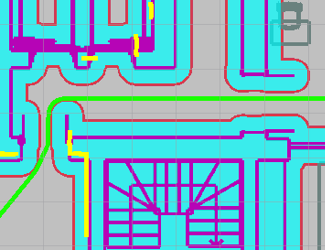
\includegraphics[width=0.98\textwidth, height=5.5cm]{costmap_not_inflated.png}\\
        }
        % {\sourcecitation{Autor}.}
    \end{subfigure}
    \begin{subfigure}{0.5\linewidth}
        {
            \centering
            \caption{Mapa de custo com inflação alta.}
            \label{fig:inflation_high}
            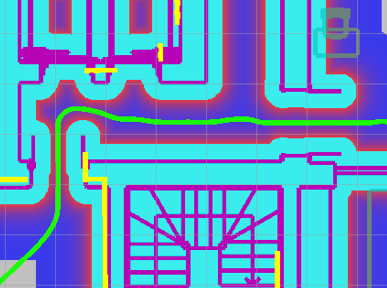
\includegraphics[width=0.98\textwidth, height=5.5cm]{costmap_inflated.png}\\
        }
        % {\sourcecitation{Autor}.}
    \end{subfigure}
\end{figure}

\begin{figure}[h]
    \caption{Mapeamento de obstáculos da camada \textit{voxel}}
    \begin{subfigure}{0.5\linewidth}
        {
            \centering
            \caption{Mapa de custo antes da detecção do obstáculo.}
            \label{fig:voxel_before}
            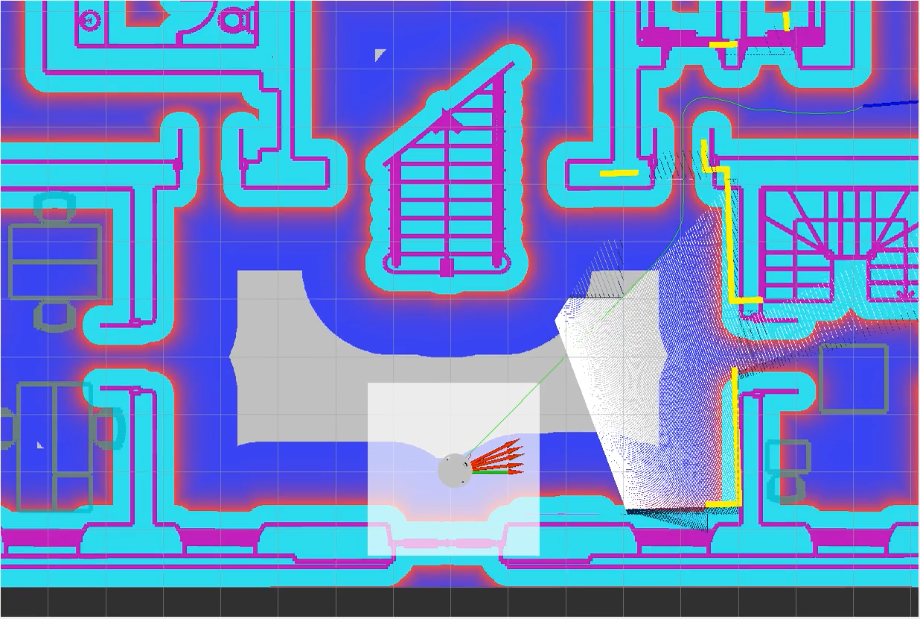
\includegraphics[width=0.98\textwidth]{costmap_voxel_before.png}\\
        }
        % {\sourcecitation{Autor}.}
    \end{subfigure}
    \begin{subfigure}{0.5\linewidth}
        {
            \centering
            \caption{Mapa de custo após a detecção do obstáculo.}
            \label{fig:voxel_after}
            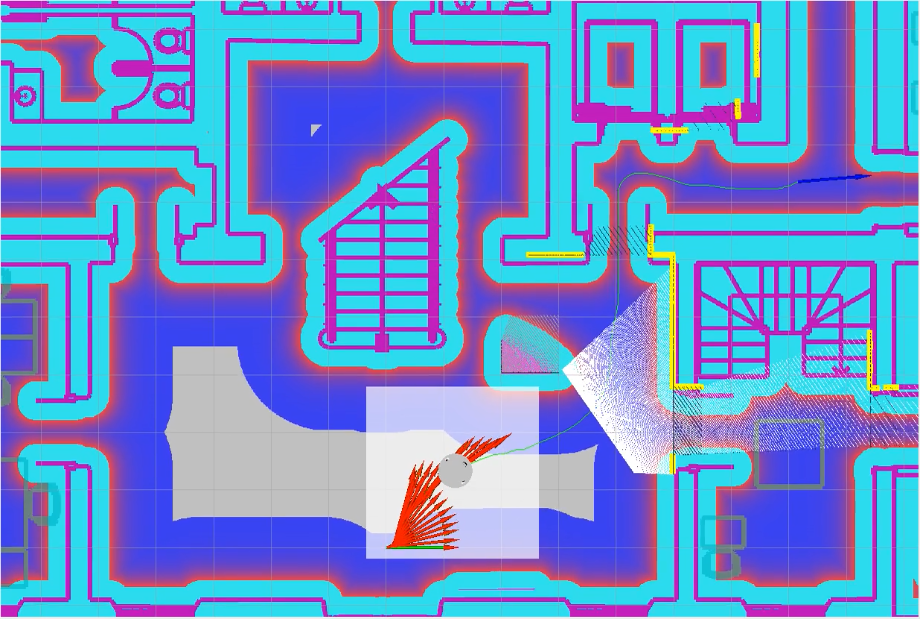
\includegraphics[width=0.98\textwidth]{costmap_voxel_after.png}\\
        }
        % {\sourcecitation{Autor}.}
    \end{subfigure}
\end{figure}

\section{Odometria, localização e mapeamento SLAM}

O testes de odometria, localização e mapeamento SLAM foram realizados na mesma
sacola de dados, como descrito na seção \ref{met:testes},
permitindo dessa forma, a mesma entrada em cada sistema.

Na Figura \ref{fig:base_bag}, é mostrado o robô realizando a trajetória
de testes. As setas em vermelho representam a mensagem de odometria do
robô, onde é indicado a posição e orientação do robô. A linha verde indica
a trajetória planejada do robô.
O caminho realizado neste teste começa na origem, segue em direção a porta
no canto superior direto da sala, percorre o corredor e entra na primeira
sala.
É possível comparar a percepção de diferentes ambientes neste teste, como
em corredores estreitos e salas abertas.

Devido ao tamanho da sacola de dados em razão da captura das imagens
da câmera, não foi possível realizar uma simulação longa, que percorresse
uma grande área do mapa e retornasse ao ponto inicial, testando assim o
fechamento de laço, que é um ponto importante no mapeamento de sistemas
SLAM.

\begin{figure}[h]
    {
        \centering
        \caption{Robô durante o teste realizado.}
        \label{fig:base_bag}
        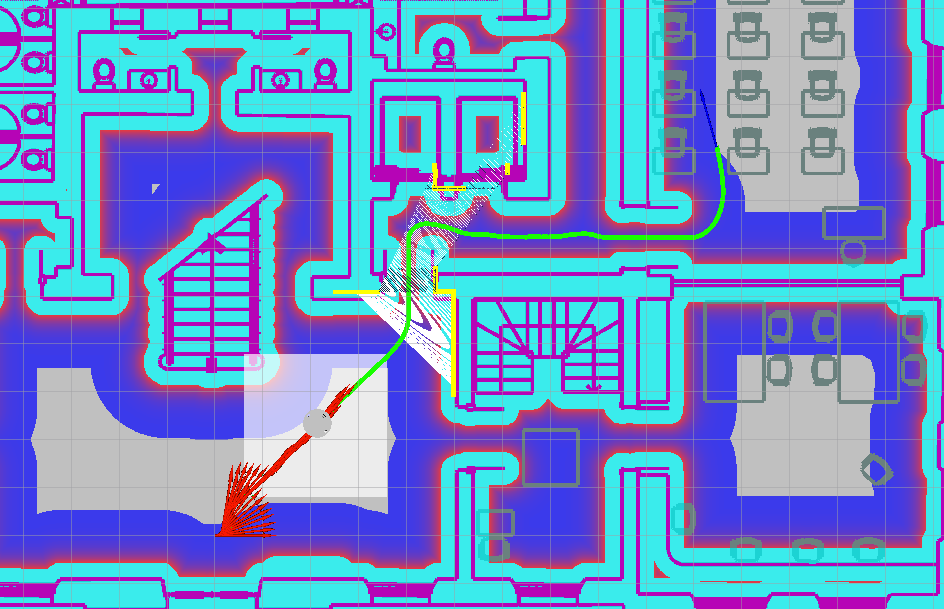
\includegraphics[width=0.9\textwidth]{base_bag_sim_zoom.png}\\
    }
    % {\sourcecitation{Autor}.}
\end{figure}

Após o fim da simulação e captura de dados, foram executados os
sistemas de odometria na sacola gerada.
Neste teste, utilizou-se a transformada estática entre os sistemas
de coordenadas \texttt{map} e \texttt{odom}, para comparar a odometria
das rodas e visual.
Na Figura \ref{fig:odom}, são mostrados as estimativas da posição do robô
nos eixos X e Y em relação a origem do sistema de coordenadas \texttt{map}
dos dois sistemas de odometria em verde, comparados com a posição real do
robô em vermelho.

A odometria das rodas, mostrada na Figura \ref{fig:odom_controller},
mostra grande divergência em relação a posição real do robô, com essa
divergência enviesada para a direita.
Este resultado não é esperado, e indica alguma falha no sistema de odometria
das rodas, podendo ser causada pela descrição do robô.
\todo{acho que seria uma boa referenciar um artigo que diga a divergencia
    esperada da odometria das rodas}

Por outro lado, a odometria visual, mostrada na Figura \ref{fig:odom_visual},
apresentou um resultado satisfatório. Existe uma divergência ao longo do tempo,
além de um erro significativo na última curva da trajetória, estimando um caminho
com alto ruído.
Porém, esta odometria apresentou desempenho satisfatório para utilização
em conjuntos com os testes dos sistemas de SLAM.
Porém, este desempenho pode não ser replicado em ambientes reais, devido
ao ruído presente fora da simulação.

\begin{figure}[h]
    \caption{Sistemas de odometria}
    \label{fig:odom}
    \begin{subfigure}{0.5\linewidth}
        {
            \centering
            \caption{Odometria das rodas.}
            \label{fig:odom_controller}
            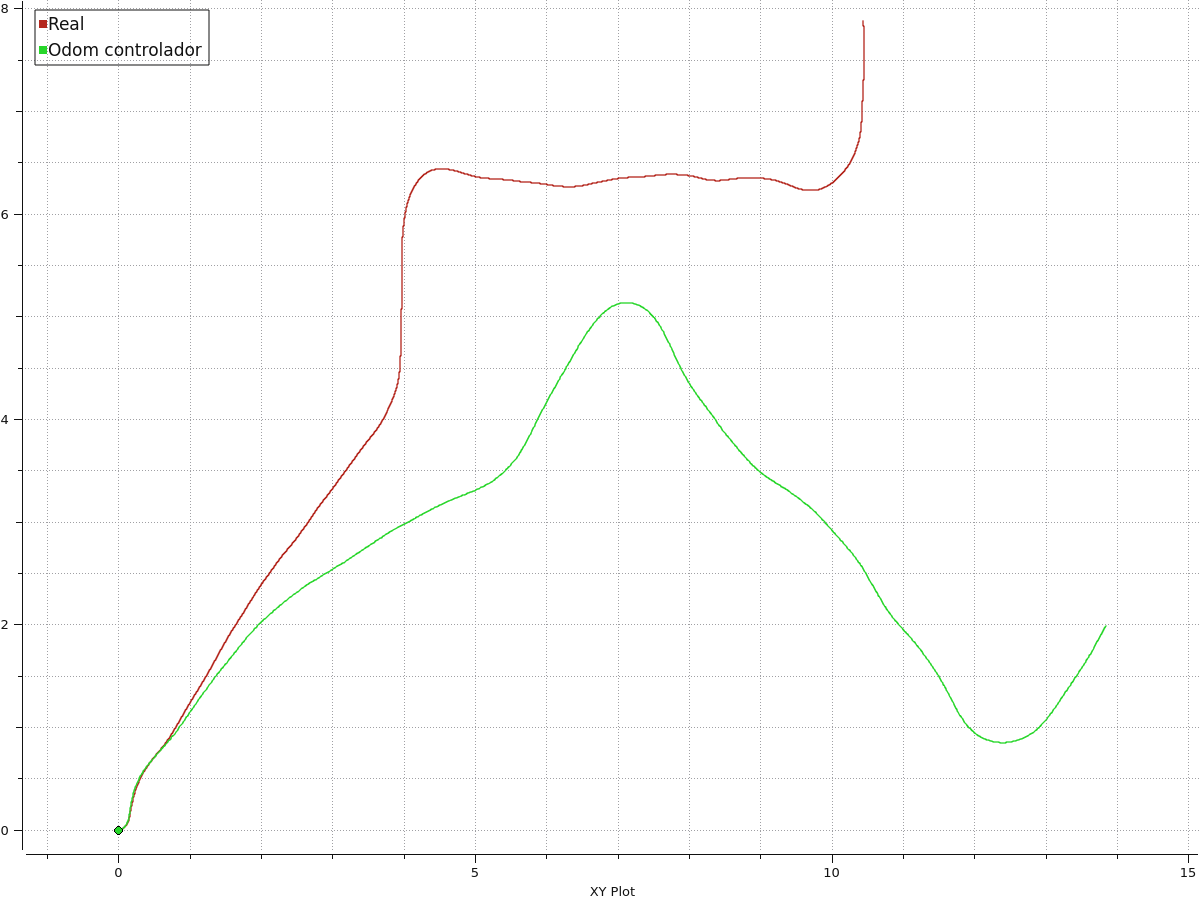
\includegraphics[width=0.98\linewidth]{odom-controlador.png}\\
        }
        % {\sourcecitation{Autor}.}
    \end{subfigure}
    \begin{subfigure}{0.5\linewidth}
        {
            \centering
            \caption{Odometria visual.}
            \label{fig:odom_visual}
            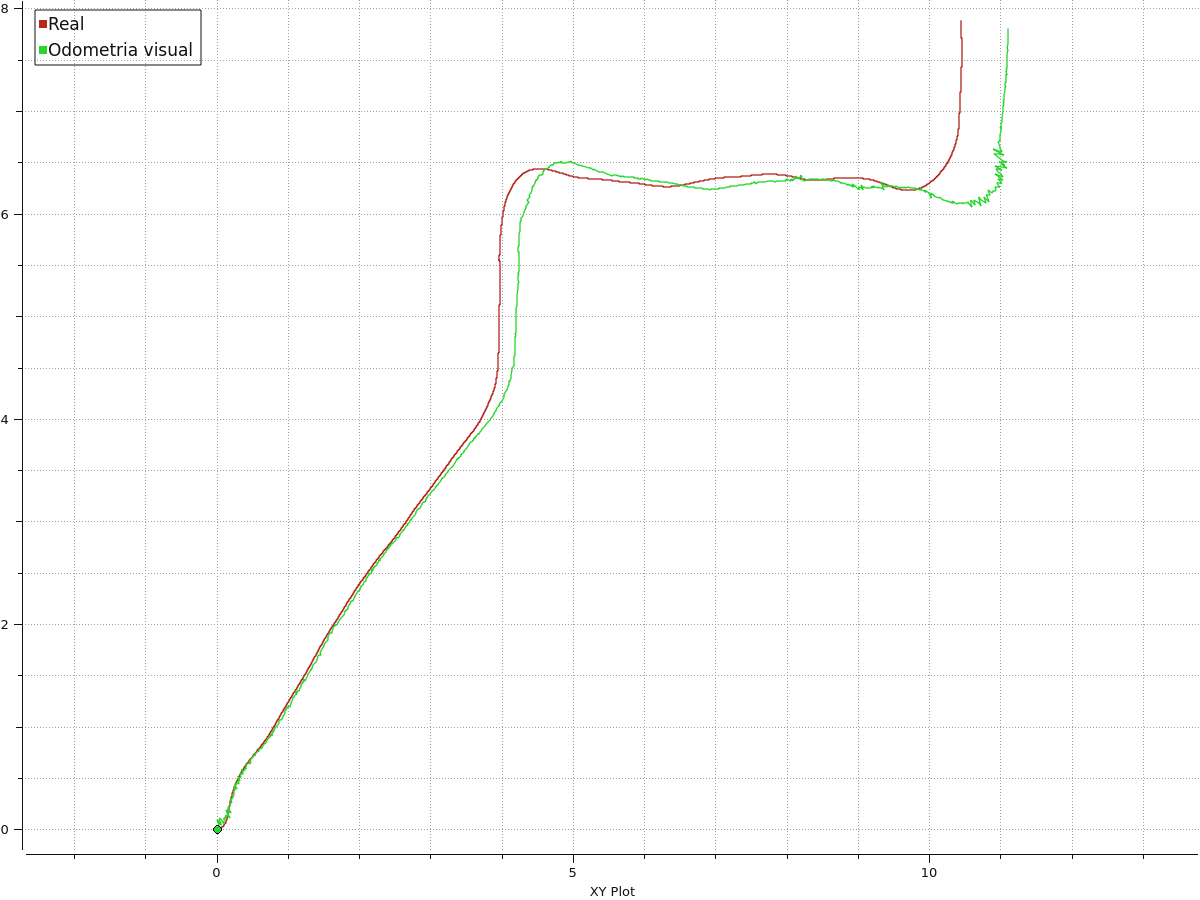
\includegraphics[width=0.98\linewidth]{odom-visual.png}\\
        }
        % {\sourcecitation{Autor}.}
    \end{subfigure}
\end{figure}


\begin{figure}[h]
    \caption{Sistemas de localização}
    \begin{subfigure}{0.5\linewidth}
        {
            \centering
            \caption{Pacote \texttt{rtabmap\_slam}.}
            \label{fig:localization_rtabmap}
            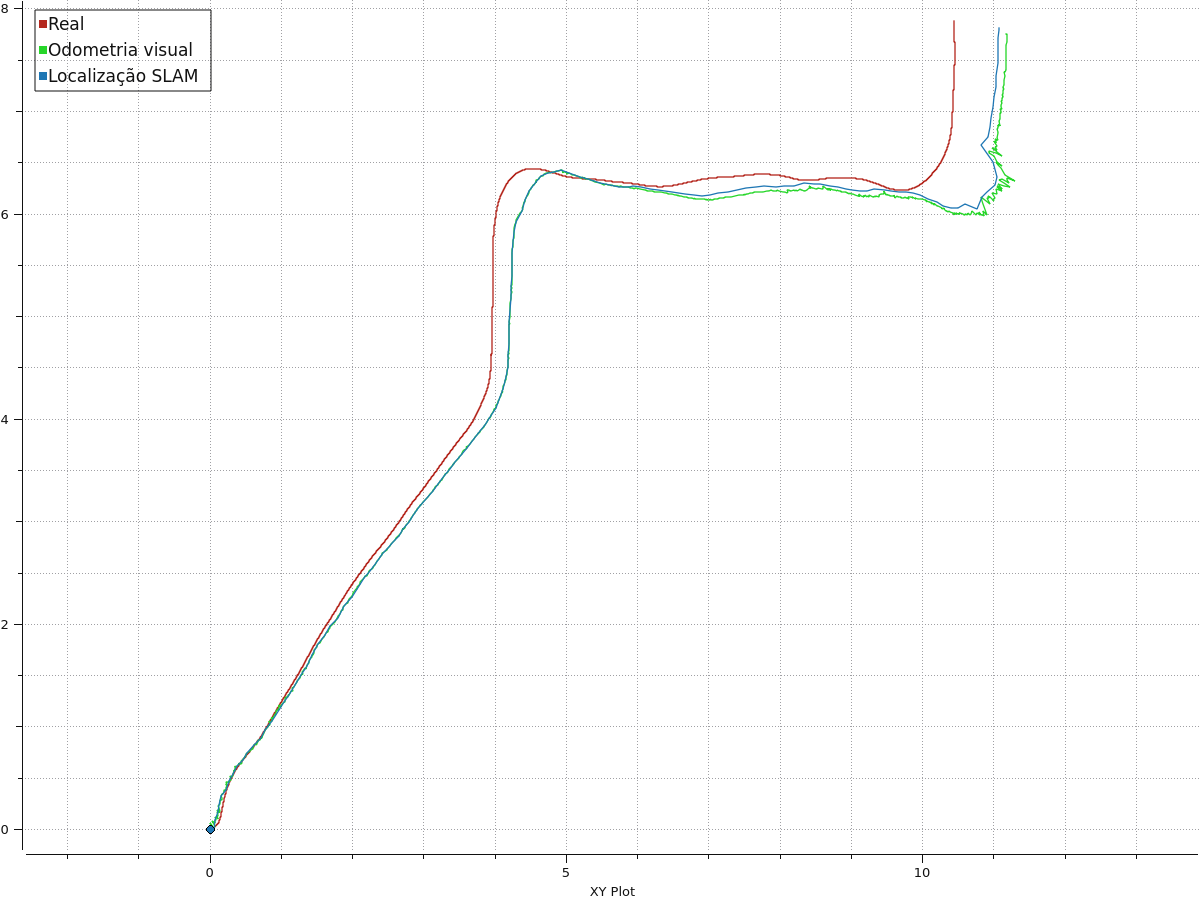
\includegraphics[width=0.98\linewidth]{localization-rtabmap.png}\\
        }
        % {\sourcecitation{Autor}.}
    \end{subfigure}
    \begin{subfigure}{0.5\linewidth}
        {
            \centering
            \caption{Pacote \texttt{slam\_toolbox}.}
            \label{fig:localization_slam_toolbox}
            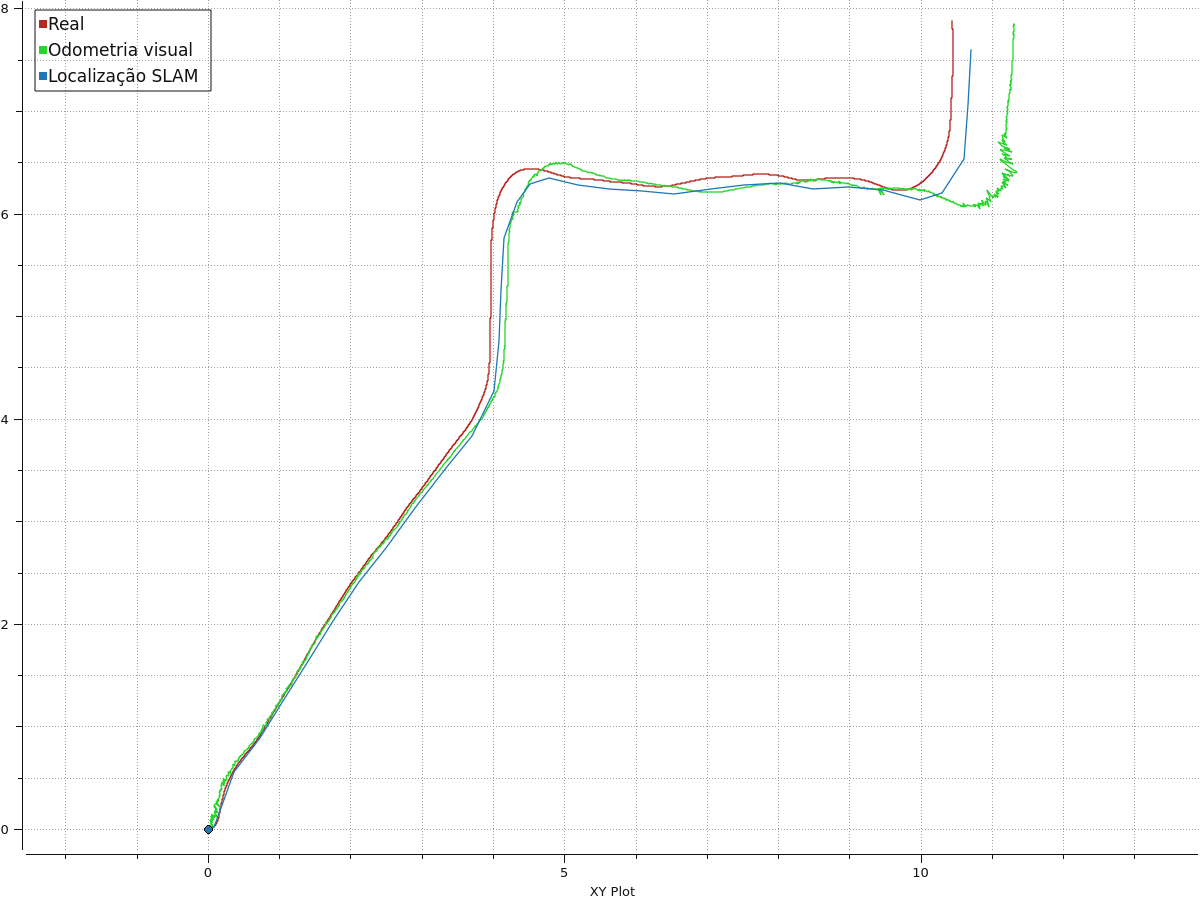
\includegraphics[width=0.98\linewidth]{localization-slam-toolbox.png}\\
        }
        % {\sourcecitation{Autor}.}
    \end{subfigure}
\end{figure}

\todo[inline]{colocar que, devido ao processamento e meu note nao ser tao bom
    a odometria visual nao ficou igual em todas as execucoes mesmo com a mesma
    entrada}
% \begin{figure}[h]
%     \caption{Mapeamento SLAM}
%     \begin{subfigure}{0.5\linewidth}
%         {
%             \centering
%             \caption{Pacote \texttt{rtabmap\_slam}.}
%             \label{fig:mapping_rtabmap}
%             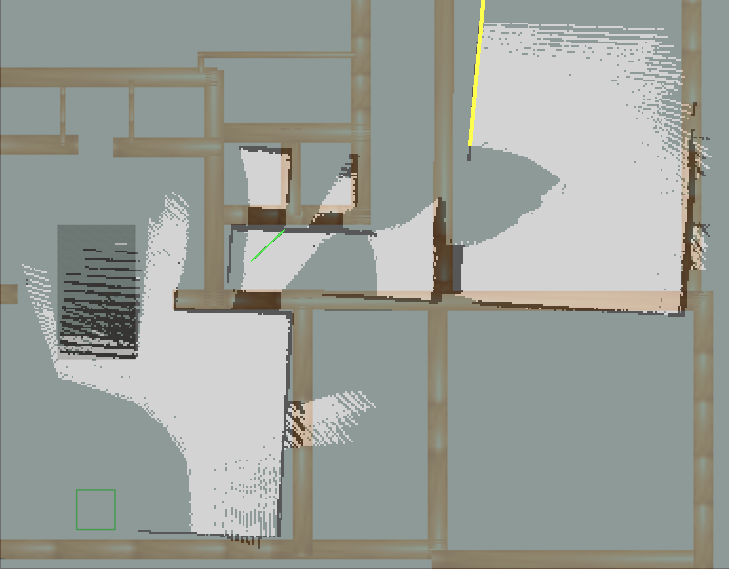
\includegraphics[width=0.98\linewidth]{rtabmap_slam_map-compared.png}\\
%         }
%         {\sourcecitation{Autor}.}
%     \end{subfigure}
%     \begin{subfigure}{0.5\linewidth}
%         {
%             \centering
%             \caption{Pacote \texttt{slam\_toolbox}.}
%             \label{fig:mapping_slam_toolbox}
%             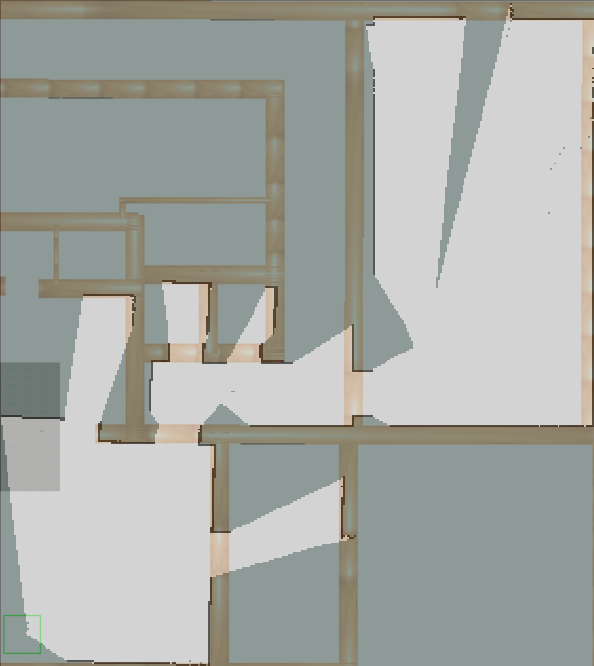
\includegraphics[width=0.98\linewidth]{slam_toolbox_map-compared.png}\\
%         }
% {\sourcecitation{Autor}.}
%     \end{subfigure}
% \end{figure}

\begin{figure}[h]
    {
        \centering
        \caption{Pacote \texttt{rtabmap\_slam}.}
        \label{fig:mapping_rtabmap}
        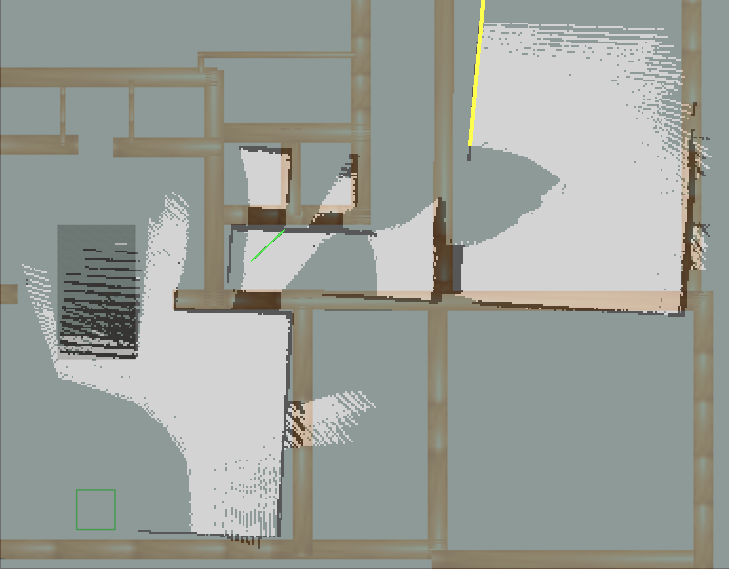
\includegraphics[width=0.6\linewidth]{rtabmap_slam_map-compared.png}\\
    }
    % {\sourcecitation{Autor}.}
\end{figure}

\begin{figure}[h]
    {
        \centering
        \caption{Pacote \texttt{slam\_toolbox}.}
        \label{fig:mapping_slam_toolbox}
        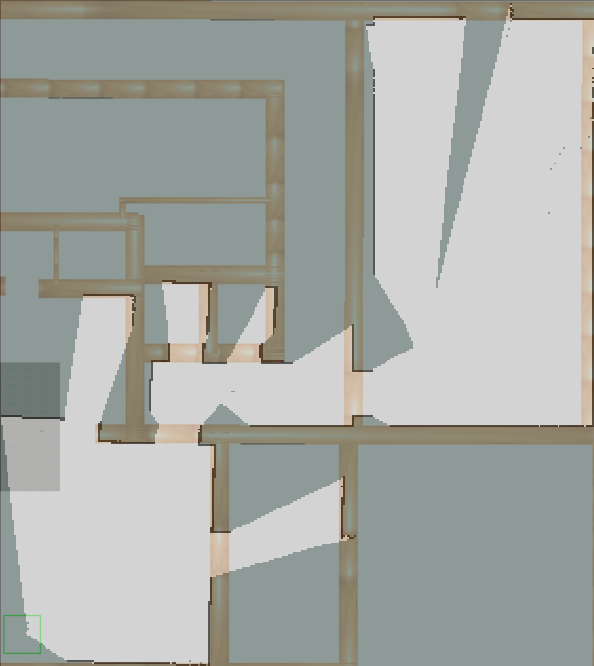
\includegraphics[width=0.6\linewidth]{slam_toolbox_map-compared.png}\\
    }
    % {\sourcecitation{Autor}.}
\end{figure}



\chapter{Conclusão}
\label{conclusao}


\printbibliography

%\begin{appendix}
%
%\end{appendix}
%
%
%\begin{annex}
%\end{annex}

\end{document}

